% =====================================================================
% Relatório técnico - Trabalho Individual II - SCOM
% Compilar com XeLaTeX (dentro de docs/relatorio):
%   latexmk -xelatex relatorio.tex
% =====================================================================
\documentclass[12pt,a4paper]{article}

\usepackage{fontspec}
\setmonofont{DejaVu Sans Mono}[Scale=0.8]
\usepackage{polyglossia}
\setdefaultlanguage[variant=brazilian]{portuguese}
\gappto\captionsportuguese{\renewcommand{\contentsname}{Índice}}

\usepackage[top=3cm,bottom=2.5cm,left=3cm,right=2.5cm]{geometry}
\usepackage{graphicx}
\usepackage{float}
\usepackage{caption}
\usepackage{booktabs}
\usepackage{longtable}
\usepackage{tabularx}
\usepackage{array}
\usepackage{enumitem}
\usepackage{xcolor}
\usepackage{listings}
\usepackage{fvextra}
\usepackage{titlesec}
\usepackage{tikz}
\usetikzlibrary{positioning,arrows.meta,fit,shapes.multipart}
\usepackage{amssymb}
\usepackage{newunicodechar}
\newunicodechar{≥}{\ensuremath{\geq}}
\newunicodechar{≤}{\ensuremath{\leq}}
\newunicodechar{→}{\ensuremath{\rightarrow}}
\usepackage[hidelinks]{hyperref}

\setlength{\parindent}{1.25cm}
\setlength{\parskip}{0.3em}
\renewcommand{\arraystretch}{1.25}
\captionsetup{font=small}
\setcounter{secnumdepth}{3}
\titleformat{\paragraph}[hang]{\normalfont\normalsize\bfseries\ttfamily}{}{0pt}{}
\titlespacing*{\paragraph}{0pt}{1.2ex}{0.6ex}
\setlength{\emergencystretch}{3em}
\providecommand{\tightlist}{\setlength{\itemsep}{0pt}\setlength{\parskip}{0pt}}

\definecolor{fundo}{HTML}{F6F6F6}
\definecolor{comentario}{HTML}{6A737D}
\lstset{
  basicstyle=\ttfamily\footnotesize,
  backgroundcolor=\color{fundo},
  frame=single, rulecolor=\color{black!25},
  breaklines=true, breakatwhitespace=false,
  columns=fullflexible, keepspaces=true,
  showstringspaces=false, tabsize=2,
  commentstyle=\color{comentario},
  xleftmargin=2pt, xrightmargin=2pt
}
\lstdefinelanguage{JS}{
  keywords={const,let,async,await,return,if,else,throw,new,export,import,from,function,for,of},
  sensitive=true, comment=[l]{//}, morecomment=[s]{/*}{*/}, morestring=[b]', morestring=[b]`
}

\newcommand{\cod}[1]{\texttt{#1}}
\newcommand{\ok}{$\checkmark$}
\newcommand{\nao}{--}

\begin{document}

% --------------------------------------------------------------- Capa
\begin{titlepage}
  \centering
  {\bfseries UNIVERSIDADE ESTADUAL PAULISTA ``JÚLIO DE\\ MESQUITA FILHO''\\
  CAMPUS DE SOROCABA\\[0.8em]
  CURSO DE ENGENHARIA DE CONTROLE E AUTOMAÇÃO\par}
  \vfill
  {\Large\bfseries VITOR CORREIA MENDES\par}
  \vfill
  {\LARGE Trabalho Individual II -- SCOM\par}
  {\large Backend, persistência e segurança: \textit{Cuphead Boss Guide}\par}
  \vfill\vfill
  {\bfseries SOROCABA\\2026\par}
\end{titlepage}

\tableofcontents
\newpage

% =====================================================================
\section{Introdução}

Este relatório documenta a segunda etapa do projeto \textit{Cuphead Boss Guide},
desenvolvido para a disciplina SCOM. No Trabalho Individual I foi construída uma
interface web estática (HTML5 e CSS3) com estratégias para os chefes do jogo
\textit{Cuphead} e um checklist de conquistas. O Trabalho II evolui esse sistema
para uma aplicação cliente-servidor completa, acrescentando backend funcional,
persistência em banco de dados relacional, autenticação, controle de acesso por
perfis, validação de entradas, proteções de segurança, testes automatizados,
registro de logs e documentação da API.

A solução foi implementada com Node.js e Express no backend
(\textit{JavaScript everywhere}, como sugerido no enunciado) e PostgreSQL como
banco de dados. A interface do Trabalho I foi preservada visualmente e passou a
consumir a API por meio de JavaScript em módulos nativos, sem frameworks.

\begin{table}[H]
\centering
\caption{Resumo da solução}
\small
\begin{tabular}{@{}ll@{}}
\toprule
Aspecto & Escolha \\
\midrule
Frontend & HTML5, CSS3 e JavaScript (módulos ES), sem frameworks \\
Backend & Node.js 22 + Express 4, arquitetura em camadas \\
Banco de dados & PostgreSQL (testado na versão 16), driver \cod{pg} \\
Autenticação & Sessão no servidor, bcrypt e token CSRF \\
Testes & \cod{node:test} + supertest: 56 testes automatizados \\
Repositório & \url{https://github.com/akavirto123/scom-projeto-cuphead} \\
\bottomrule
\end{tabular}
\end{table}

% =====================================================================
\section{Evolução em relação ao Trabalho 1}

O Trabalho I apontava, em sua seção de limitações, que o formulário ``Sugerir Nova
Tática'' era apenas demonstrativo e que o checklist de conquistas não guardava o
progresso do usuário. Ambas as limitações foram resolvidas. A
Tabela~\ref{tab:evolucao} resume a evolução.

\begin{table}[H]
\centering
\caption{Comparação entre o Trabalho I e o Trabalho II}
\label{tab:evolucao}
\begin{tabularx}{\linewidth}{@{}>{\raggedright}p{3.2cm}>{\raggedright}X>{\raggedright\arraybackslash}X@{}}
\toprule
Item & Trabalho I (\cod{v1.0}) & Trabalho II (\cod{v2.0}) \\
\midrule
Chefes & 19 cartões fixos no HTML & Tabela no banco; listagem paginada, filtro por ilha e busca; CRUD pelo administrador \\
Formulário de tática & Sem efeito (\cod{action="\#"}) & Grava a tática como pendente; moderação pelo administrador; táticas aprovadas aparecem no card do chefe \\
Conquistas & Lista estática & Catálogo no banco e progresso salvo por usuário, com barra de percentual \\
Usuários & Inexistentes & Cadastro, login, logout e três perfis (visitante, jogador, administrador) \\
Páginas & \cod{index.html} & \cod{index.html}, \cod{conta.html} e \cod{admin.html} \\
Organização & Dois arquivos na raiz & \cod{frontend/}, \cod{backend/} e \cod{docs/} \\
Qualidade & Lighthouse e W3C & Testes automatizados, testes de segurança, logs e medição de desempenho \\
\bottomrule
\end{tabularx}
\end{table}

A identidade visual (paleta ``Vermelho Cuphead'' e ``Amarelo Vintage'', fundo de
pergaminho, fontes Bangers e Outfit) foi mantida, e os novos componentes
(formulários de login, tabelas do painel, selos de status) foram estilizados com
as mesmas variáveis CSS do Trabalho I. Duas mudanças de layout foram feitas: o
cabeçalho fixo passou a valer apenas a partir de 768\,px, porque no celular, com a
nova área de login, ele ocupava quase metade da tela; e os cartões de chefes
passaram a ser paginados (6 por página) em vez de exibidos todos de uma vez.

\begin{figure}[H]
\centering
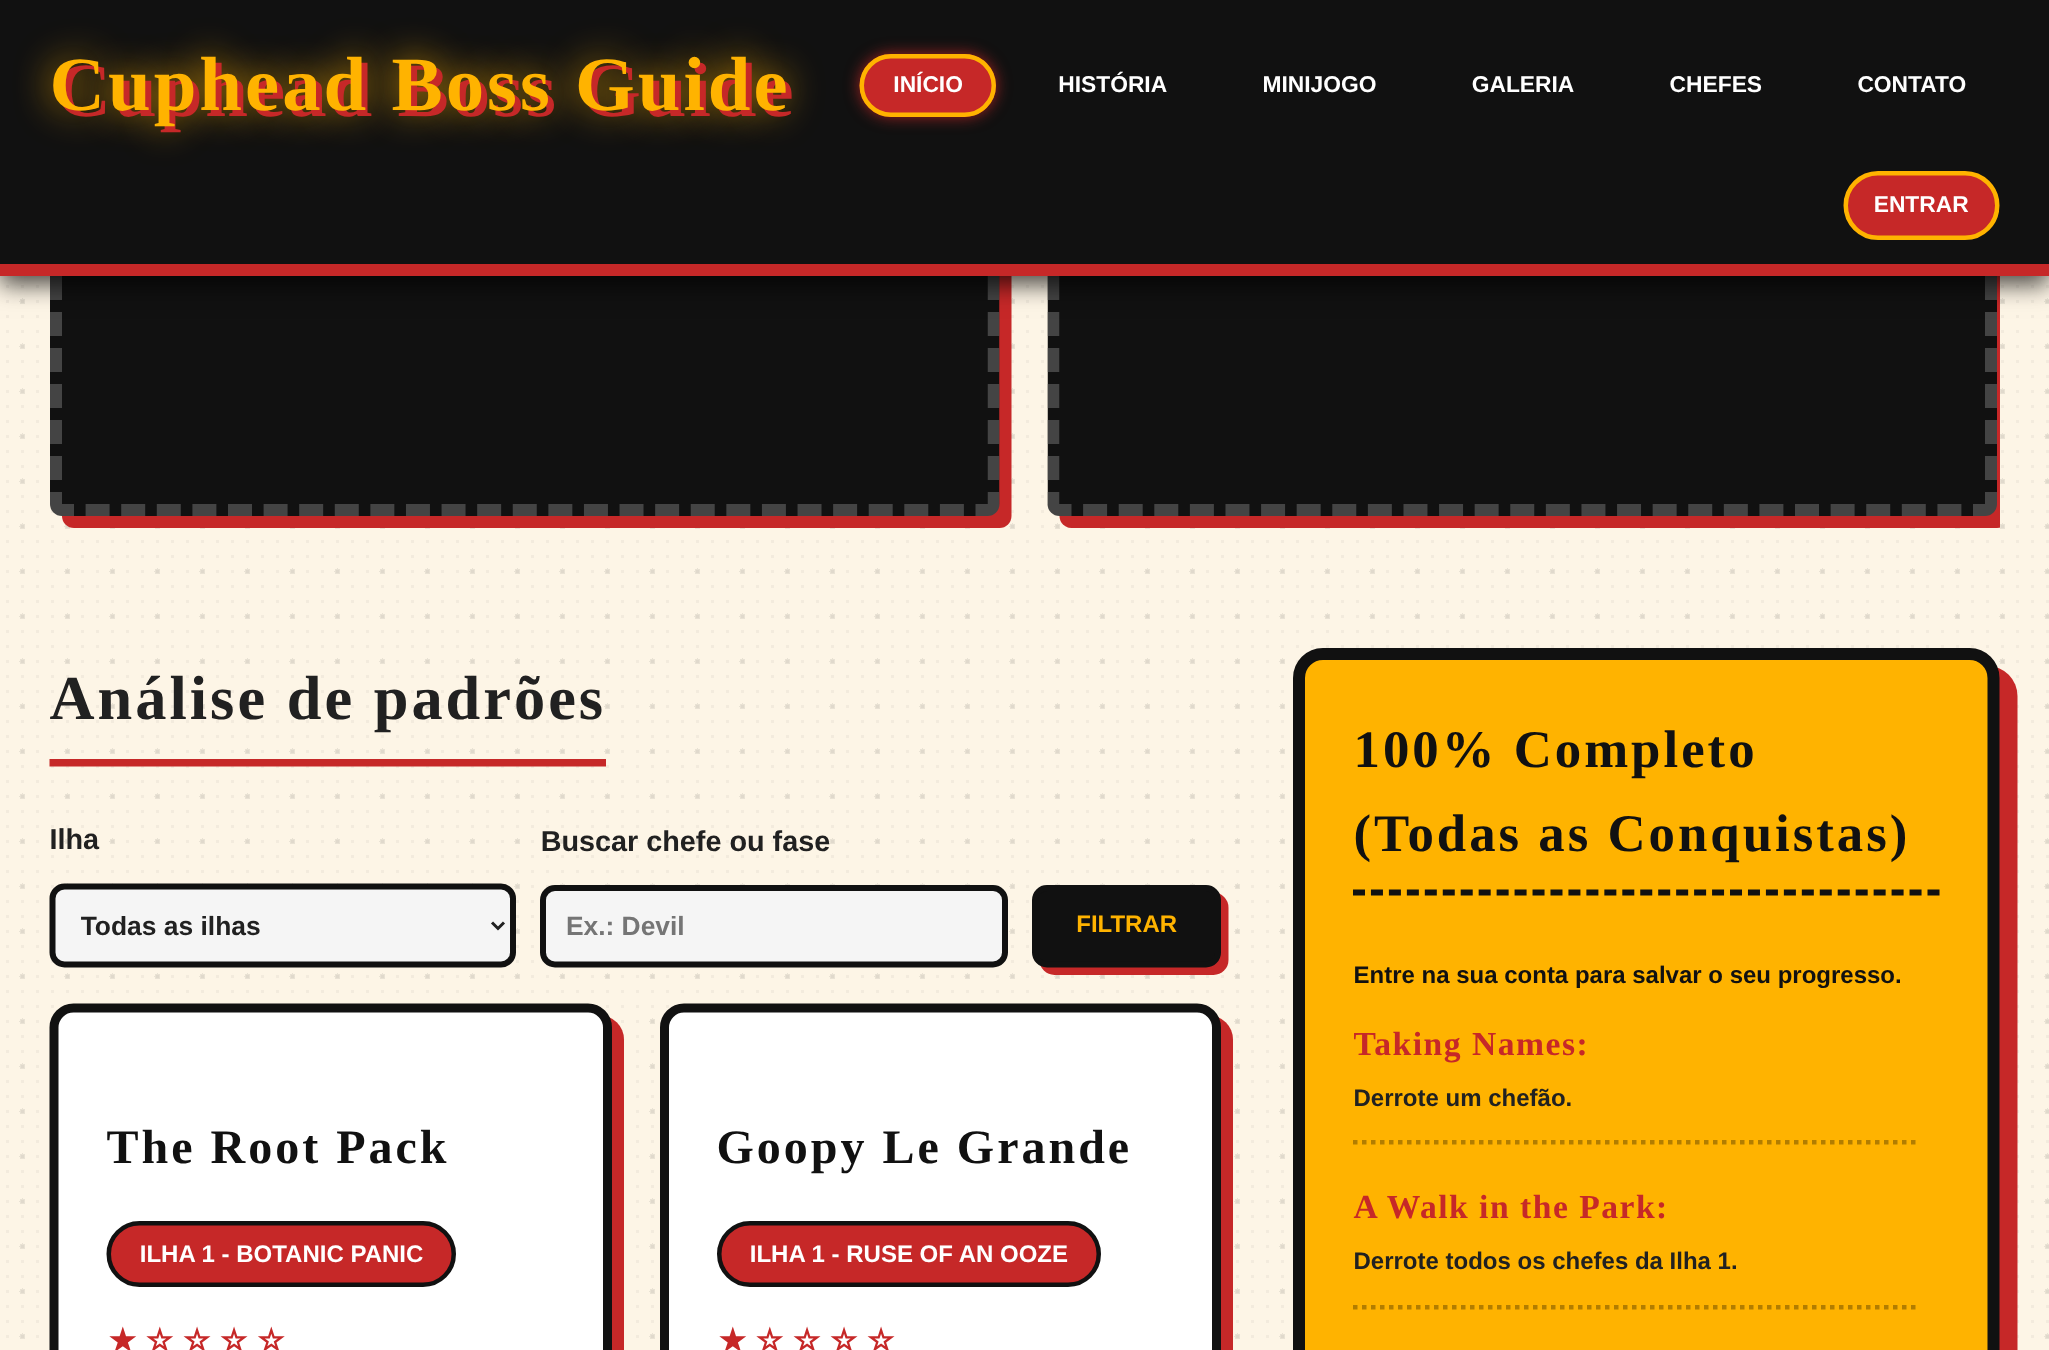
\includegraphics[width=0.92\linewidth]{../evidencias/capturas/13_desktop_chefes.png}
\caption{Página inicial do Trabalho II: filtros, cartões vindos da API e checklist de conquistas}
\end{figure}

% =====================================================================
\section{Requisitos funcionais}

\begin{longtable}{@{}l>{\raggedright}p{8.6cm}>{\raggedright\arraybackslash}p{3cm}@{}}
\caption{Requisitos funcionais e perfis envolvidos}\\
\toprule
ID & Requisito & Perfil \\
\midrule
\endfirsthead
\toprule
ID & Requisito & Perfil \\
\midrule
\endhead
RF01 & Listar chefes com paginação, filtro por ilha e busca por nome ou fase & Todos \\
RF02 & Exibir detalhes de um chefe e as táticas aprovadas da comunidade & Todos \\
RF03 & Cadastrar conta (perfil jogador por padrão) & Visitante \\
RF04 & Entrar e sair do sistema & Visitante / logado \\
RF05 & Enviar tática para um chefe (nasce como pendente) & Jogador, admin \\
RF06 & Ver, editar e excluir as próprias táticas enquanto pendentes & Jogador, admin \\
RF07 & Marcar e desmarcar conquistas e ver o percentual concluído & Jogador, admin \\
RF08 & Cadastrar, editar e excluir chefes & Admin \\
RF09 & Moderar táticas: listar por status, aprovar, rejeitar e excluir & Admin \\
RF10 & Listar usuários e alterar o perfil de outro usuário & Admin \\
RF11 & Consultar a saúde da API e do banco & Todos \\
\bottomrule
\end{longtable}

Requisitos não funcionais atendidos: senhas armazenadas apenas como hash bcrypt;
toda entrada validada no backend; respostas JSON padronizadas; registro de eventos
com \textit{timestamp}; configuração por variáveis de ambiente; execução local com
três comandos (\cod{npm install}, \cod{npm run db:migrar}, \cod{npm start}).

% =====================================================================
\section{Arquitetura do sistema}

Foi adotada uma arquitetura cliente-servidor com o backend organizado em
\textbf{camadas}. A ``visão'' é o frontend estático, que consome a API JSON; o
backend é dividido em camada HTTP (rotas e controllers), camada de lógica de
aplicação (services, regras de domínio e validação) e camada de acesso a dados
(repositories). Cada camada depende apenas da camada imediatamente abaixo:
controllers não escrevem SQL, repositories não conhecem objetos de requisição e
services não sabem que existe HTTP.

\begin{figure}[H]
\centering
\resizebox{\linewidth}{!}{%
\begin{tikzpicture}[
  camada/.style={draw, rounded corners=2pt, minimum width=11.5cm, minimum height=0.95cm, align=center, font=\small},
  rotulo/.style={font=\footnotesize\itshape, anchor=west},
  seta/.style={-{Latex[length=2mm]}, thick}]
  \node[camada, fill=yellow!25] (front) {\textbf{frontend/}: index.html, conta.html, admin.html, css/, js/ (api.js, dom.js, ...)};
  \node[camada, fill=gray!10, below=0.9cm of front] (mw) {\textbf{middlewares/}: helmet (CSP) $\rightarrow$ id da requisição $\rightarrow$ rate limit $\rightarrow$ sessão $\rightarrow$ CSRF $\rightarrow$ permissão};
  \node[camada, fill=red!8, below=0.35cm of mw] (http) {\textbf{routes/} + \textbf{controllers/}: URL e método $\rightarrow$ chamada ao service $\rightarrow$ resposta JSON};
  \node[camada, fill=red!15, below=0.35cm of http] (serv) {\textbf{services/} + \textbf{domain/} + \textbf{validators/}: regras de negócio, validação, permissões};
  \node[camada, fill=red!25, below=0.35cm of serv] (repo) {\textbf{repositories/}: SQL parametrizado (\$1, \$2, ...)};
  \node[camada, fill=blue!10, below=0.9cm of repo, minimum width=4cm] (db) {\textbf{PostgreSQL}};
  \draw[seta] (front) -- node[right, font=\footnotesize]{HTTP/JSON, cookie de sessão, X-CSRF-Token} (mw);
  \draw[seta] (repo) -- node[right, font=\footnotesize]{pool de conexões (pg)} (db);
  \node[draw, dashed, rounded corners, fit=(mw)(repo), inner sep=6pt, label={[font=\footnotesize]north east:backend/src (Express)}] {};
  \node[rotulo] at ([xshift=0.5cm]http.east) {Interface HTTP};
  \node[rotulo] at ([xshift=0.5cm]serv.east) {Lógica};
  \node[rotulo] at ([xshift=0.5cm]repo.east) {Dados};
\end{tikzpicture}}
\caption{Camadas da aplicação}
\label{fig:camadas}
\end{figure}

\subsection{Organização dos diretórios}

\begin{lstlisting}
scom-projeto-cuphead/
|-- frontend/            interface (arquivos estáticos)
|   |-- index.html  conta.html  admin.html
|   |-- css/style.css
|   `-- js/              api.js, dom.js, cabecalho.js, inicio.js, conta.js, admin.js
|-- backend/
|   |-- src/
|   |   |-- server.js    ponto de entrada
|   |   |-- app.js       composition root: liga as camadas
|   |   |-- config/      env.js, database.js, logger.js
|   |   |-- middlewares/ sessao, csrf, autorizacao, limitadores, tratadorErros
|   |   |-- routes/  controllers/  services/  repositories/
|   |   |-- validators/  esquemas de entrada
|   |   |-- domain/      permissoes.js (matriz RBAC)
|   |   `-- utils/       AppError, validacao, http
|   |-- database/        migrations/, script_completo.sql, executor
|   |-- scripts/         criarAdmin.js, benchmark.js, demonstrar-seguranca.sh
|   |-- tests/           unit/ e integracao/
|   `-- .env.example
`-- docs/                API.md, ARQUITETURA.md, CHECKLIST.md, evidencias/, relatorio/
\end{lstlisting}

\subsection{Injeção de dependências}

Cada módulo exporta uma \textit{fábrica}, por exemplo
\cod{criarChefeService(\{ chefeRepository, ilhaRepository, logger \})}. O arquivo
\cod{app.js} é o único ponto que instancia e conecta as camadas. Com isso, os
testes unitários substituem os repositories por versões em memória e os testes de
integração montam a aplicação real com outra configuração (banco de testes,
\textit{rate limit} menor e um logger que captura os eventos).

\subsection{Fluxo de uma requisição}

Tomando como exemplo um jogador enviando uma tática (\cod{POST /api/taticas}):
(1) o \cod{helmet} aplica os cabeçalhos de segurança; (2) é gerado um
\cod{requisicaoId}; (3) o corpo JSON é lido com limite de 10\,KB; (4) a sessão é
carregada do PostgreSQL pelo cookie; (5) o usuário da sessão é buscado no banco;
(6) o token CSRF do cabeçalho é comparado com o da sessão; (7) a matriz de
permissões é consultada; (8) o controller chama \cod{taticaService.criar}; (9) o
service valida e sanitiza os dados, confere se o chefe existe, grava pelo
repository e registra o evento \cod{entidade.criada}; (10) qualquer exceção em
qualquer etapa é convertida em resposta JSON pelo tratador central de erros.

% =====================================================================
\section{Modelo de dados}

O banco possui oito tabelas. A entidade principal é \cod{chefes}; \cod{taticas} e
\cod{usuario\_conquistas} registram a participação dos usuários. A
Figura~\ref{fig:er} mostra os relacionamentos.

\begin{figure}[H]
\centering
\resizebox{\linewidth}{!}{%
\begin{tikzpicture}[
  tab/.style={rectangle split, rectangle split parts=2, draw, rounded corners=1pt, font=\scriptsize, align=left, inner sep=3pt, rectangle split part fill={red!20,white}},
  fk/.style={-{Latex[length=2mm]}, thick}]
  \node[tab] (usu) {\textbf{usuarios}\nodepart{two}PK id\\nome, email (UNIQUE)\\senha\_hash, perfil\\criado\_em};
  \node[tab, right=1.6cm of usu] (tat) {\textbf{taticas}\nodepart{two}PK id\\FK chefe\_id, FK usuario\_id\\FK moderado\_por\\conteudo, status\\criado\_em, atualizado\_em};
  \node[tab, right=1.6cm of tat] (che) {\textbf{chefes}\nodepart{two}PK id\\nome (UNIQUE), fase\\FK ilha\_id, FK criado\_por\\estrategia, dificuldade\\criado\_em, atualizado\_em};
  \node[tab, below=1.4cm of che] (ilh) {\textbf{ilhas}\nodepart{two}PK id\\nome (UNIQUE)\\ordem (UNIQUE)};
  \node[tab, below=1.4cm of usu] (uc) {\textbf{usuario\_conquistas}\nodepart{two}PK (usuario\_id, conquista\_id)\\FK usuario\_id, FK conquista\_id\\concluida\_em};
  \node[tab, right=1.6cm of uc] (con) {\textbf{conquistas}\nodepart{two}PK id\\nome (UNIQUE)\\descricao, ordem};
  \node[tab, below=0.6cm of uc, xshift=-0.3cm] (ses) {\textbf{sessoes}\nodepart{two}PK sid\\sess, expire};
  \node[tab, right=0.6cm of ses] (mig) {\textbf{schema\_migrations}\nodepart{two}PK nome, aplicada\_em};
  \draw[fk] (tat) -- node[above,font=\tiny]{N:1} (usu);
  \draw[fk] (tat) -- node[above,font=\tiny]{N:1} (che);
  \draw[fk] (che) -- node[right,font=\tiny]{N:1} (ilh);
  \draw[fk] (uc) -- node[left,font=\tiny]{N:1} (usu);
  \draw[fk] (uc) -- node[above,font=\tiny]{N:1} (con);
  \draw[fk, dashed] (che.north) to[bend right=25] node[above,font=\tiny]{criado\_por} (usu.north);
\end{tikzpicture}}
\caption{Modelo entidade-relacionamento (setas apontam para a tabela referenciada)}
\label{fig:er}
\end{figure}

\begin{table}[H]
\centering
\caption{Constraints e índices}
\small
\begin{tabularx}{\linewidth}{@{}l>{\raggedright\arraybackslash}X@{}}
\toprule
Tipo & Aplicação \\
\midrule
PRIMARY KEY & Todas as 8 tabelas (\cod{usuario\_conquistas} usa PK composta) \\
FOREIGN KEY & 7 FKs: \cod{ON DELETE CASCADE} para táticas e progresso, \cod{RESTRICT} para ilha do chefe, \cod{SET NULL} para autor/moderador \\
UNIQUE & e-mail do usuário, nome do chefe, nome e ordem da ilha, nome e ordem da conquista \\
NOT NULL & Todas as colunas obrigatórias \\
CHECK & perfil $\in$ \{jogador, admin\}; e-mail em minúsculas; dificuldade 1--5; status $\in$ \{pendente, aprovada, rejeitada\}; tamanhos de nome, estratégia e conteúdo \\
Índices & \cod{chefes(ilha\_id)}, \cod{chefes(lower(nome))}, \cod{taticas(chefe\_id, status)}, \cod{taticas(usuario\_id)}, \cod{taticas(status, criado\_em)}, \cod{sessoes(expire)} \\
Trigger & \cod{definir\_atualizado\_em()} atualiza \cod{atualizado\_em} em chefes e táticas \\
\bottomrule
\end{tabularx}
\end{table}

Os tipos foram escolhidos pelo domínio: \cod{SMALLINT} para ilhas, conquistas e
dificuldade; \cod{VARCHAR(n)} com o mesmo limite usado na validação;
\cod{TIMESTAMPTZ} para datas; chaves \cod{GENERATED ALWAYS AS IDENTITY}.

\paragraph{Migrações}
O esquema é versionado em \cod{backend/database/migrations/}
(\cod{001\_criar\_tabelas.sql} e \cod{002\_dados\_iniciais.sql}, que importa os 19
chefes e 28 conquistas do HTML do Trabalho I). O comando \cod{npm run db:migrar}
aplica apenas as migrações pendentes e registra cada uma em
\cod{schema\_migrations}. O arquivo \cod{script\_completo.sql}, gerado a partir das
migrações por \cod{npm run db:script}, é o script único de criação do banco e foi
testado com \cod{psql -v ON\_ERROR\_STOP=1} em um banco vazio (Anexo~\ref{anx:sql}).

% =====================================================================
\section{Estratégia de autenticação}

Foi escolhida autenticação por \textbf{sessão no servidor} em vez de JWT. Com
sessão, o logout invalida o acesso imediatamente (o registro é apagado do banco),
e o identificador fica em um cookie \cod{HttpOnly}, inacessível ao JavaScript da
página.

\begin{itemize}[leftmargin=1.5em]
  \item \textbf{Senhas:} hash \textbf{bcrypt} com custo 12 (configurável em
  \cod{BCRYPT\_COST}) e salt aleatório embutido. A senha em texto nunca é gravada,
  registrada em log ou devolvida pela API. Política: 8+ caracteres com letras e
  números, até 72 bytes (limite do bcrypt).
  \item \textbf{Login:} e-mail inexistente e senha errada recebem a mesma resposta
  (\cod{401 CREDENCIAIS\_INVALIDAS}) e o mesmo tempo de processamento, pois o hash
  é comparado mesmo quando o usuário não existe. Isso impede descobrir quais
  e-mails estão cadastrados.
  \item \textbf{Fixação de sessão:} o id de sessão é regenerado a cada login.
  \item \textbf{Cookie:} \cod{cuphead.sid} com \cod{HttpOnly}, \cod{SameSite=Strict}
  e \cod{Secure} quando servido por HTTPS; expira após 120 minutos sem uso.
  \item \textbf{Armazenamento:} sessões na tabela \cod{sessoes} do PostgreSQL;
  sobrevivem ao reinício do servidor e são removidas no logout.
  \item \textbf{Usuário recarregado a cada requisição:} a sessão guarda só o id;
  perfil e existência da conta são lidos do banco, então uma mudança de perfil vale
  na hora.
  \item \textbf{Força bruta:} \textit{rate limit} de 5 tentativas malsucedidas por
  IP a cada 15 minutos (\cod{429}).
  \item \textbf{Logout:} \cod{POST /api/auth/logout} destrói a sessão e apaga o
  cookie; o cookie antigo passa a receber \cod{401}.
\end{itemize}

\subsection{Controle de acesso e matriz de permissões}

São três perfis: \textbf{visitante} (sem login), \textbf{jogador} (padrão no
cadastro) e \textbf{administrador}. A matriz fica em um único arquivo,
\cod{src/domain/permissoes.js}, e cada rota declara a ação que exige, por exemplo
\cod{acesso.exigirPermissao('chefe:criar')}. Visitante sem permissão recebe
\cod{401}; usuário logado sem permissão recebe \cod{403}. Ações não listadas são
negadas por padrão.

\begin{table}[H]
\centering
\caption{Matriz de permissões}
\label{tab:matriz}
\small
\begin{tabularx}{\linewidth}{@{}>{\raggedright}Xccc@{}}
\toprule
Ação (identificador na matriz) & Visitante & Jogador & Admin \\
\midrule
Listar e ver chefes e ilhas (\cod{chefe:listar}) & \ok & \ok & \ok \\
Criar, editar e excluir chefe (\cod{chefe:criar/editar/excluir}) & \nao & \nao & \ok \\
Ver táticas aprovadas (\cod{tatica:listar\_aprovadas}) & \ok & \ok & \ok \\
Enviar tática (\cod{tatica:criar}) & \nao & \ok & \ok \\
Ver as próprias táticas (\cod{tatica:listar\_proprias}) & \nao & \ok & \ok \\
Editar/excluir a própria tática pendente (\cod{tatica:editar\_propria}) & \nao & \ok & \ok \\
Moderar táticas (\cod{tatica:moderar}) & \nao & \nao & \ok \\
Ver conquistas (\cod{conquista:listar}) & \ok & \ok & \ok \\
Marcar o próprio progresso (\cod{conquista:marcar\_progresso}) & \nao & \ok & \ok \\
Listar usuários (\cod{usuario:listar}) & \nao & \nao & \ok \\
Alterar perfil de outro usuário (\cod{usuario:alterar\_perfil}) & \nao & \nao & \ok \\
\bottomrule
\end{tabularx}
\end{table}

Regras que dependem do registro, e não só do perfil, ficam no service: o jogador
só altera táticas das quais é autor e apenas enquanto estão pendentes
(\cod{403}/\cod{409}); o administrador não pode alterar o próprio perfil, para não
perder o acesso por engano.

% =====================================================================
\section{Estratégia de segurança}

\begin{longtable}{@{}>{\raggedright}p{3cm}>{\raggedright}p{7.6cm}>{\raggedright\arraybackslash}p{3.3cm}@{}}
\caption{Ameaças e mitigações}\\
\toprule
Ameaça & Mitigação & Onde \\
\midrule
\endfirsthead
\toprule
Ameaça & Mitigação & Onde \\
\midrule
\endhead
SQL Injection & Todas as consultas usam parâmetros posicionais (\cod{\$1, \$2}); o texto SQL nunca é concatenado com entrada do usuário. Curingas do \cod{LIKE} são escapados. Ids de rota são validados como inteiros. & \cod{repositories/}, \cod{validacao.js} \\
XSS refletido e armazenado & A API responde só JSON com \cod{X-Content-Type-Options: nosniff}. O frontend insere dados apenas com \cod{textContent}/nós de texto (nenhum \cod{innerHTML}). \textit{Content Security Policy} com \cod{script-src 'self'} bloqueia scripts e estilos inline. & \cod{js/dom.js}, \cod{app.js} \\
CSRF & Token de 256 bits por sessão, exigido no cabeçalho \cod{X-CSRF-Token} em POST/PUT/PATCH/DELETE e comparado em tempo constante; cookie \cod{SameSite=Strict}. & \cod{middlewares/csrf.js} \\
Acesso não autorizado & Middleware de permissão em todas as rotas protegidas; regras de autoria no service. & \cod{autorizacao.js} \\
\textit{Mass assignment} & A validação só aceita campos descritos no esquema; enviar \cod{"perfil":"admin"} no cadastro é ignorado. & \cod{validacao.js} \\
Força bruta & \textit{Rate limit} no login e na API. & \cod{limitadores.js} \\
Vazamento de informação & Stack trace só em desenvolvimento; respostas nunca incluem \cod{senha\_hash}; mensagens de login genéricas; cabeçalho \cod{X-Powered-By} removido. & \cod{tratadorErros.js} \\
Entradas abusivas & Corpo limitado a 10\,KB; limites de tamanho em todos os campos; remoção de caracteres de controle e invisíveis. & \cod{app.js}, \cod{validacao.js} \\
Credenciais no código & Banco, segredo de sessão e administrador vêm do \cod{.env}, que está no \cod{.gitignore}; o repositório tem só o \cod{.env.example}. & \cod{config/env.js} \\
\textit{Clickjacking} & \cod{frame-ancestors 'none'} e \cod{X-Frame-Options}. & \cod{app.js} \\
\bottomrule
\end{longtable}

\subsection{Validação e sanitização}

Toda entrada externa (corpo, query string e parâmetros de rota) passa pela função
\cod{validar(dados, esquema)}, chamada pelos services. Cada campo declara tipo
(\cod{texto}, \cod{inteiro}, \cod{email}, \cod{senha}, \cod{opcao}), se é
obrigatório e os limites de tamanho ou valor. Textos são normalizados (Unicode NFC),
têm caracteres de controle e invisíveis removidos e espaços repetidos reduzidos;
senhas não são alteradas. Os erros são devolvidos juntos, por campo:

\begin{lstlisting}
{ "erro": { "status": 422, "codigo": "VALIDACAO",
    "mensagem": "Os dados enviados são inválidos.",
    "detalhes": [ { "campo": "nome",  "mensagem": "deve ser um texto." },
                  { "campo": "email", "mensagem": "deve ser um e-mail válido." },
                  { "campo": "senha", "mensagem": "deve ter no mínimo 8 caracteres." } ] } }
\end{lstlisting}

O banco repete as regras principais em constraints \cod{CHECK}, como última linha
de defesa; violações que chegarem até ele também são convertidas em respostas
\cod{409} ou \cod{422} pelo tratador de erros.

\subsection{Tratamento de erros}

Todas as falhas terminam no middleware \cod{tratadorErros.js}, que devolve status
HTTP, código, mensagem legível e o \cod{requisicaoId} (o mesmo registrado no log).
Erros esperados usam a classe \cod{AppError}; erros do banco e do parser JSON são
convertidos; os demais viram \cod{500 ERRO\_INTERNO}. O bloco \cod{tecnico} (nome,
mensagem original e stack trace) só é incluído com \cod{NODE\_ENV=development}
(Figura~\ref{fig:erro500}); um teste automatizado garante que ele não aparece fora
desse modo.

\begin{figure}[H]
\centering
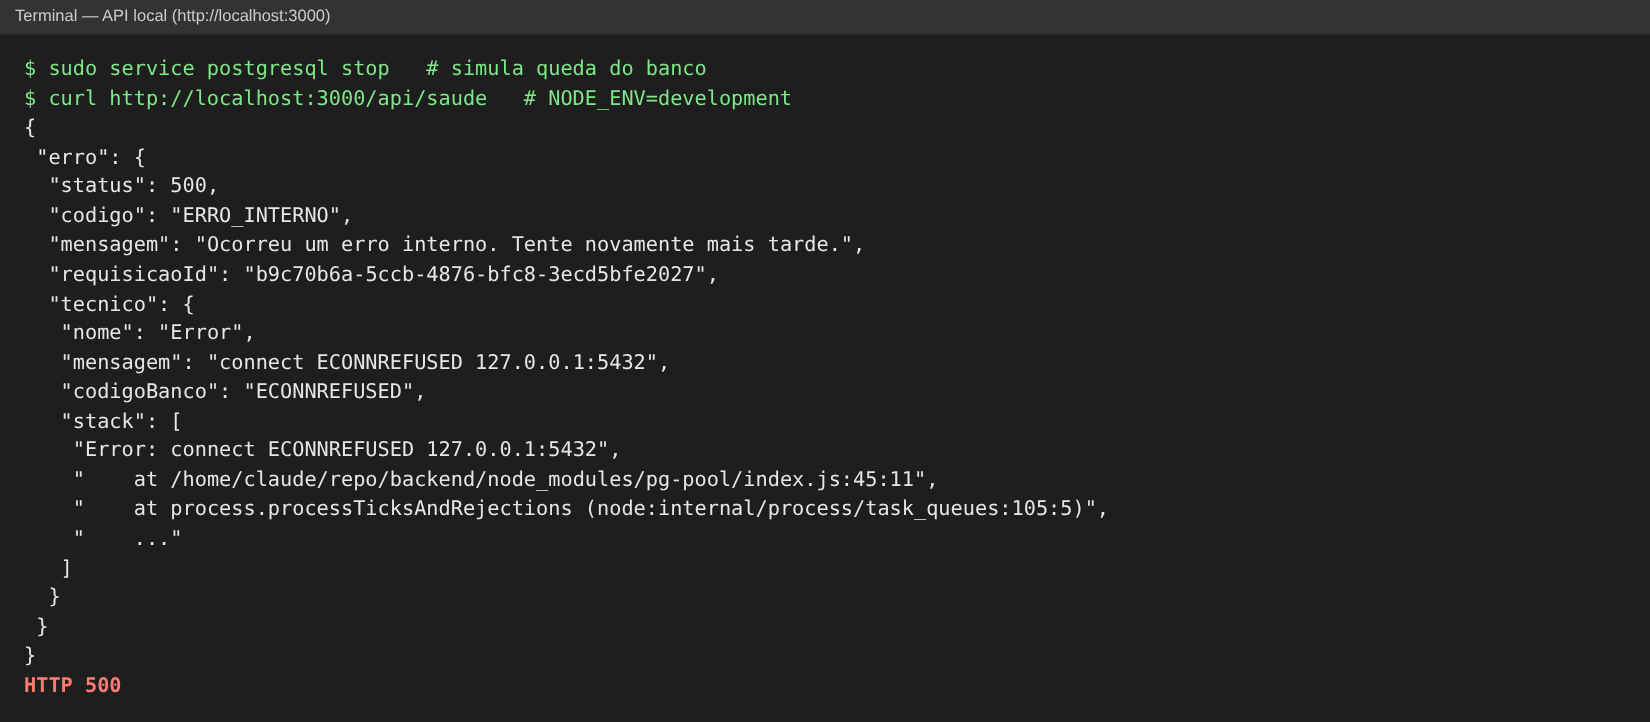
\includegraphics[width=0.85\linewidth]{../evidencias/capturas/erro500_01.png}
\caption{Erro interno em modo desenvolvimento (banco desligado de propósito): detalhes técnicos visíveis}
\label{fig:erro500}
\end{figure}

% =====================================================================
\section{Endpoints implementados}

A API possui 25 endpoints. A documentação completa (parâmetros, exemplos de
requisição e resposta e códigos de status de cada um) está em \cod{docs/API.md} e
reproduzida no Anexo~\ref{anx:api}.

\begin{longtable}{@{}l>{\raggedright}p{5.6cm}>{\raggedright}p{2.6cm}>{\raggedright\arraybackslash}p{3.4cm}@{}}
\caption{Resumo dos endpoints}\\
\toprule
Método & URL & Acesso & Sucesso / erros \\
\midrule
\endfirsthead
\toprule
Método & URL & Acesso & Sucesso / erros \\
\midrule
\endhead
GET & \cod{/api/saude} & público & 200 / 500 \\
GET & \cod{/api/auth/sessao} & público & 200 \\
POST & \cod{/api/auth/registro} & público & 201 / 403, 409, 422 \\
POST & \cod{/api/auth/login} & público & 200 / 401, 403, 422, 429 \\
POST & \cod{/api/auth/logout} & logado & 204 / 401, 403 \\
GET & \cod{/api/auth/me} & logado & 200 / 401 \\
GET & \cod{/api/ilhas} & público & 200 \\
GET & \cod{/api/chefes} & público & 200 / 422 \\
GET & \cod{/api/chefes/:id} & público & 200 / 404, 422 \\
POST & \cod{/api/chefes} & admin & 201 / 401, 403, 409, 422 \\
PUT & \cod{/api/chefes/:id} & admin & 200 / 401, 403, 404, 409, 422 \\
DELETE & \cod{/api/chefes/:id} & admin & 204 / 401, 403, 404 \\
GET & \cod{/api/chefes/:id/taticas} & público & 200 / 404, 422 \\
POST & \cod{/api/taticas} & jogador, admin & 201 / 401, 403, 422 \\
GET & \cod{/api/taticas/minhas} & jogador, admin & 200 / 401 \\
PATCH & \cod{/api/taticas/:id} & autor & 200 / 401, 403, 404, 409, 422 \\
DELETE & \cod{/api/taticas/:id} & autor ou admin & 204 / 401, 403, 404, 409 \\
GET & \cod{/api/taticas} & admin & 200 / 401, 403, 422 \\
PATCH & \cod{/api/taticas/:id/status} & admin & 200 / 401, 403, 404, 422 \\
GET & \cod{/api/conquistas} & público & 200 \\
GET & \cod{/api/conquistas/progresso} & jogador, admin & 200 / 401 \\
PUT & \cod{/api/conquistas/:id/progresso} & jogador, admin & 204 / 401, 404, 422 \\
DELETE & \cod{/api/conquistas/:id/progresso} & jogador, admin & 204 / 401, 404, 422 \\
GET & \cod{/api/usuarios} & admin & 200 / 401, 403, 422 \\
PATCH & \cod{/api/usuarios/:id/perfil} & admin & 200 / 401, 403, 404, 409, 422 \\
\bottomrule
\end{longtable}

Os métodos seguem a semântica HTTP: \cod{GET} para leitura, \cod{POST} para criar
(com cabeçalho \cod{Location}), \cod{PUT} para substituir, \cod{PATCH} para
alterações parciais e \cod{DELETE} para remover (\cod{204} sem corpo). Toda
resposta com corpo é JSON no formato \cod{\{ "dados": ... \}} ou
\cod{\{ "erro": ... \}}. Listagens aceitam \cod{?pagina=} e \cod{?limite=} e
devolvem o bloco \cod{paginacao}.

% =====================================================================
\section{Estratégia de testes}

Os testes usam o executor nativo do Node.js (\cod{node:test}) e a biblioteca
\textbf{supertest}, que faz requisições HTTP reais à aplicação Express. São dois
níveis:

\begin{itemize}[leftmargin=1.5em]
  \item \textbf{Unitários (34 testes, \cod{tests/unit/}):} testam a lógica de
  negócio sem banco de dados. Os services recebem repositórios falsos em memória,
  um \textit{hasher} instantâneo e um logger que captura eventos. Cobrem validação
  e sanitização, matriz de permissões, \cod{AuthService}, \cod{ChefeService} e
  \cod{TaticaService}.
  \item \textbf{Integração (22 testes, \cod{tests/integracao/}):} sobem a
  aplicação completa contra um banco de testes separado
  (\cod{cuphead\_guide\_test}), recriado com as mesmas migrações a cada execução.
  Cobrem CRUD de chefes, fluxo de moderação de táticas, progresso de conquistas,
  formato dos erros e os testes de segurança.
\end{itemize}

Os testes cobrem casos válidos e inválidos: dados fora do limite, tipos errados,
e-mail duplicado, nome de chefe duplicado, ilha inexistente, senha incorreta,
edição de tática já moderada, tática de outro usuário, JSON malformado e rota
inexistente, entre outros. A execução completa leva cerca de 3 segundos:

\begin{lstlisting}
$ cd backend
$ npm test               # todos (56)
$ npm run test:unit      # só unitários, sem banco
$ npm run test:relatorio # saída detalhada usada no Anexo C
\end{lstlisting}

\begin{table}[H]
\centering
\caption{Resultado da execução dos testes automatizados}
\begin{tabular}{@{}lrr@{}}
\toprule
Suíte & Testes & Aprovados \\
\midrule
Validação e sanitização (unitário) & 9 & 9 \\
Matriz de permissões (unitário) & 5 & 5 \\
AuthService (unitário) & 6 & 6 \\
ChefeService (unitário) & 7 & 7 \\
TaticaService (unitário) & 7 & 7 \\
API -- fluxos principais (integração) & 8 & 8 \\
Segurança (integração) & 11 & 11 \\
Rate limiting do login (integração) & 1 & 1 \\
Tratamento de erros (integração) & 2 & 2 \\
\midrule
\textbf{Total} & \textbf{56} & \textbf{56} \\
\bottomrule
\end{tabular}
\end{table}

A saída completa da execução está no Anexo~\ref{anx:testes}.

% =====================================================================
\section{Resultados dos testes de segurança}

Os testes de segurança foram feitos de duas formas: automatizados (suíte
``Segurança'', executada a cada \cod{npm test}) e manuais, com \cod{curl} contra o
servidor local, pelo script \cod{backend/scripts/demonstrar-seguranca.sh}, que
gera as capturas abaixo. A Tabela~\ref{tab:seg} resume os resultados.

\begin{longtable}{@{}>{\raggedright}p{3.1cm}>{\raggedright}p{4.6cm}>{\raggedright}p{2.6cm}>{\raggedright\arraybackslash}p{3.6cm}@{}}
\caption{Testes de segurança}\label{tab:seg}\\
\toprule
Teste & Ataque & Esperado & Obtido \\
\midrule
\endfirsthead
\toprule
Teste & Ataque & Esperado & Obtido \\
\midrule
\endhead
1. SQL Injection (login) & \cod{' OR '1'='1' --} no e-mail e na senha & Não autenticar & \cod{422} (e-mail inválido) e \cod{401} (chegou ao banco como texto) \\
1b. SQL Injection (busca) & \cod{'; DROP TABLE chefes; --} & Tratar como texto & \cod{200}, lista vazia; tabela intacta (19 chefes) \\
2. XSS & Tag \cod{<script>} em uma tática e \cod{<img onerror>} na busca & Não executar & Exibido como texto; nenhum \cod{alert}; JSON com \cod{nosniff} e CSP \\
3. CSRF & POST com cookie válido e sem token & Bloquear & \cod{403 CSRF\_INVALIDO} \\
4. Acesso sem login & \cod{GET /api/taticas/minhas} & Bloquear & \cod{401 NAO\_AUTENTICADO} \\
5. Perfil insuficiente & Jogador: \cod{DELETE /api/chefes/1}, \cod{GET /api/usuarios} & Bloquear & \cod{403 ACESSO\_NEGADO} \\
6. Sessão inválida & Reusar cookie após logout & Bloquear & \cod{401} \\
7. Força bruta & Várias senhas erradas & Limitar & \cod{429} após 5 falhas \\
\bottomrule
\end{longtable}

\begin{figure}[H]
\centering
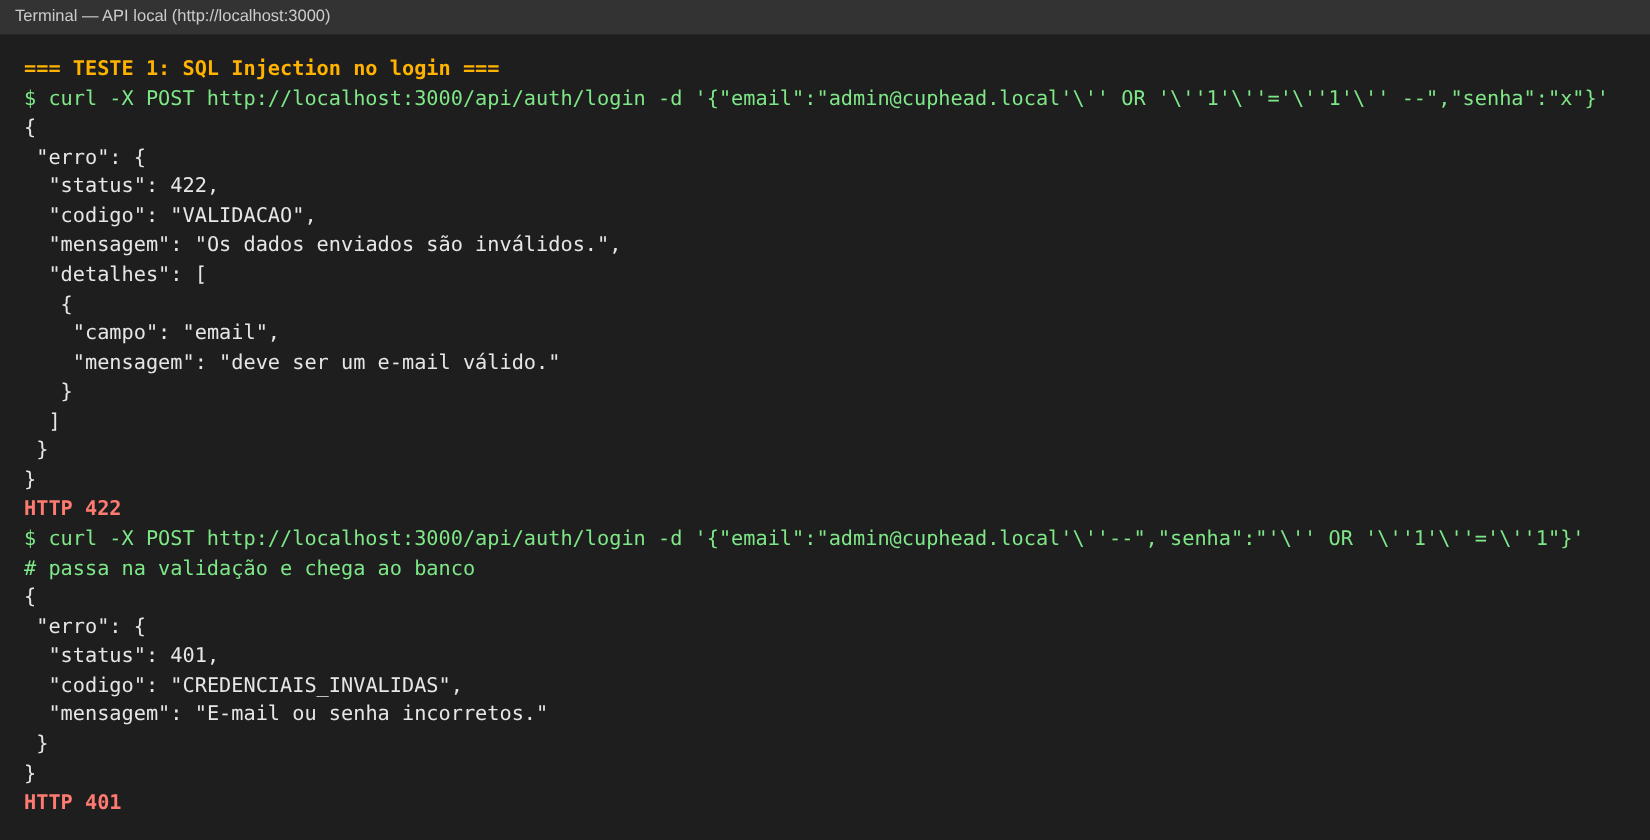
\includegraphics[width=0.9\linewidth]{../evidencias/capturas/seg_01.png}
\caption{Teste 1: SQL Injection no login. A primeira tentativa é barrada pela validação; a segunda passa na validação, chega ao banco como parâmetro e não autentica}
\end{figure}

\begin{figure}[H]
\centering
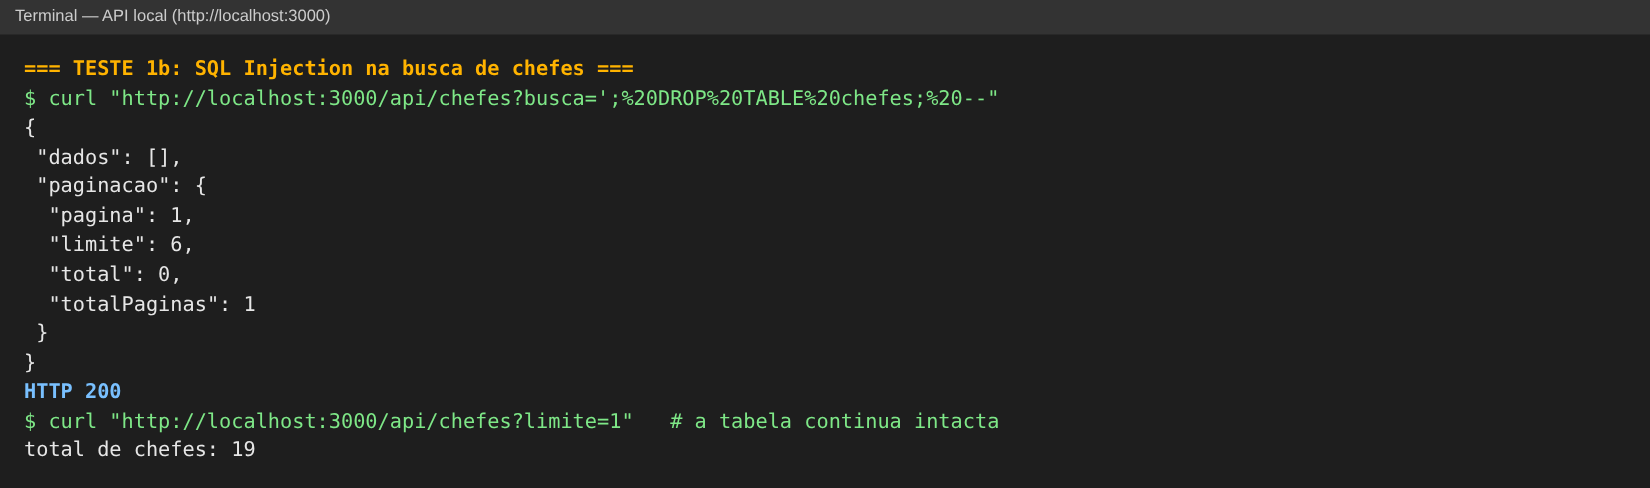
\includegraphics[width=0.9\linewidth]{../evidencias/capturas/seg_02.png}
\caption{Teste 1b: SQL Injection na busca. O texto é procurado literalmente e a tabela continua com 19 chefes}
\end{figure}

\begin{figure}[H]
\centering
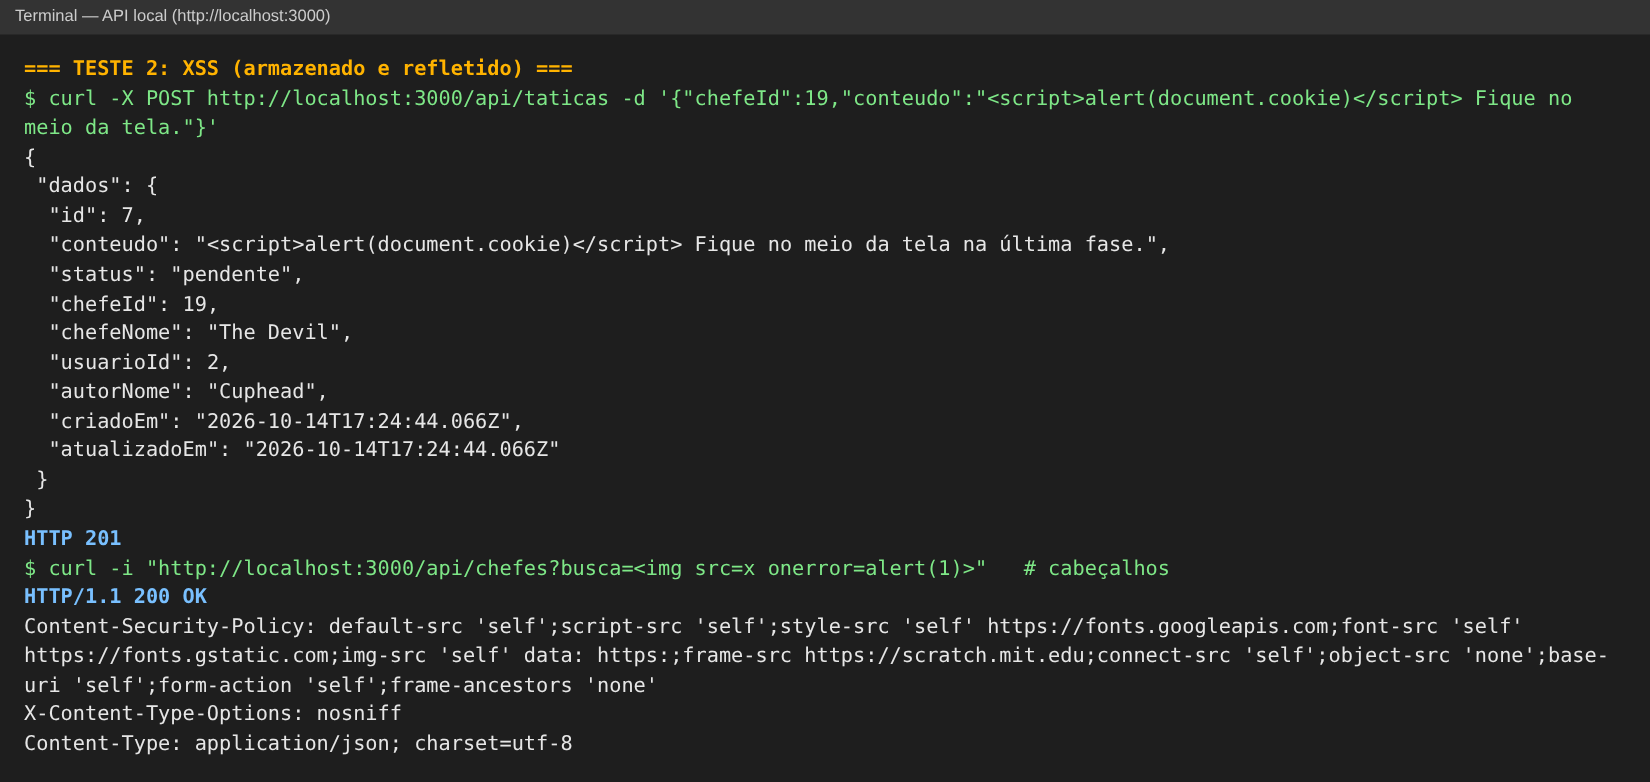
\includegraphics[width=0.9\linewidth]{../evidencias/capturas/seg_03.png}
\caption{Teste 2: XSS. O conteúdo é aceito e armazenado como texto; respostas são JSON com \cod{nosniff} e CSP}
\end{figure}

\begin{figure}[H]
\centering
\begin{minipage}[t]{0.42\linewidth}
  \centering
  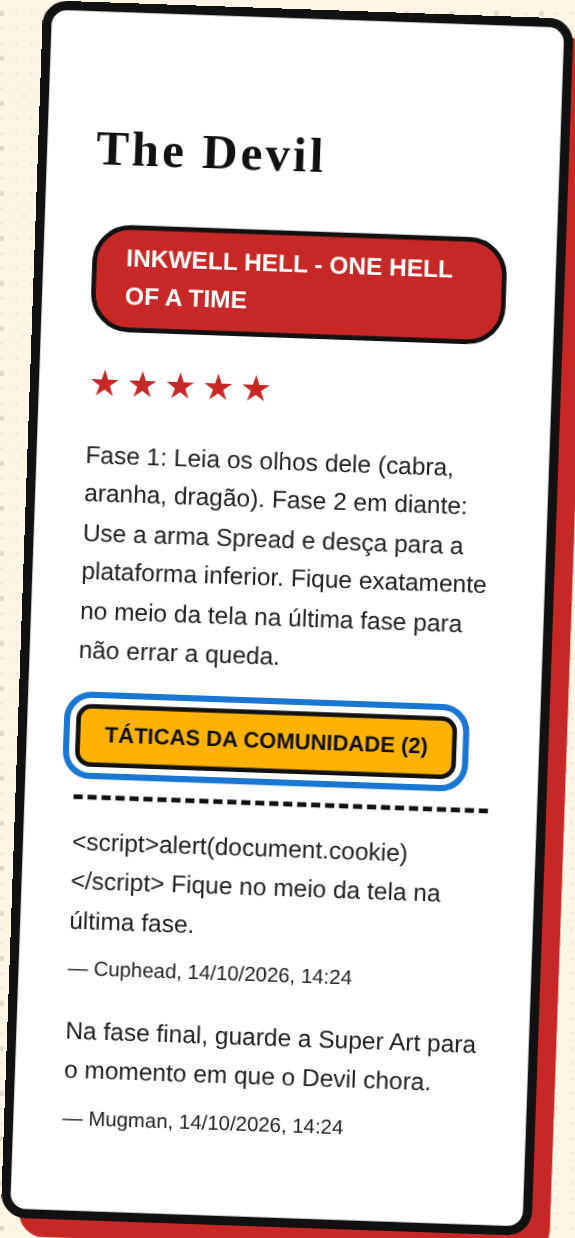
\includegraphics[width=\linewidth]{../evidencias/capturas/04_xss_exibido_como_texto.png}
  \caption{Teste 2 no navegador: a tática maliciosa aparece como texto e nenhum \cod{alert} é disparado}
  \label{fig:xss}
\end{minipage}\hfill
\begin{minipage}[t]{0.54\linewidth}
  \centering
  
\includegraphics[width=\linewidth]{../evidencias/capturas/07_jogador_no_admin_negado.png}
  \caption{Teste 5 na interface: jogador abrindo \cod{admin.html}. A API também responde \cod{403}}
\end{minipage}
\end{figure}

\begin{figure}[H]
\centering
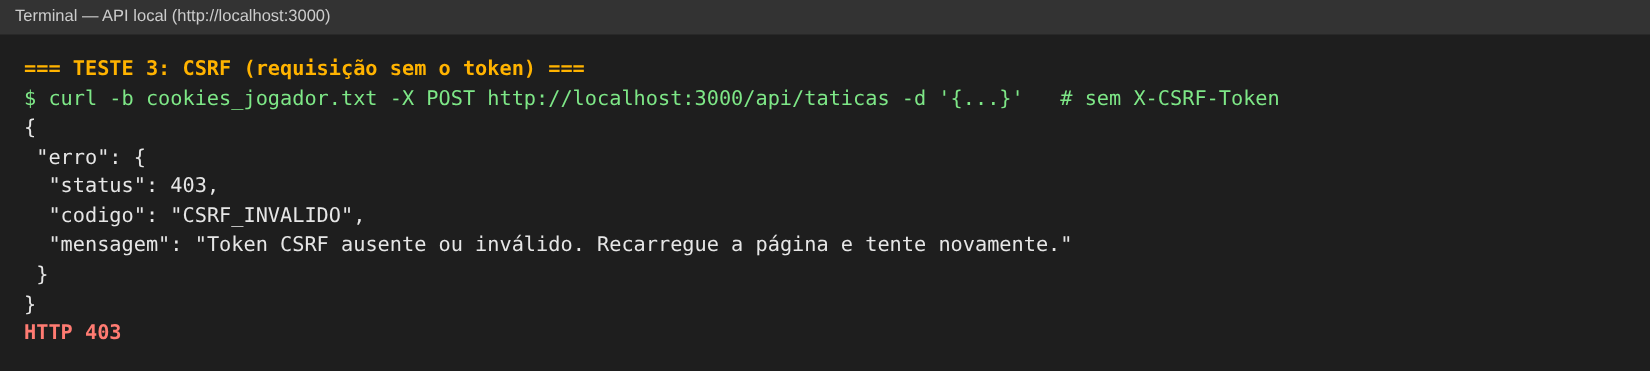
\includegraphics[width=0.9\linewidth]{../evidencias/capturas/seg_04.png}
\caption{Teste 3: CSRF. Requisição com o cookie de sessão válido, mas sem o token, é recusada}
\end{figure}

\begin{figure}[H]
\centering
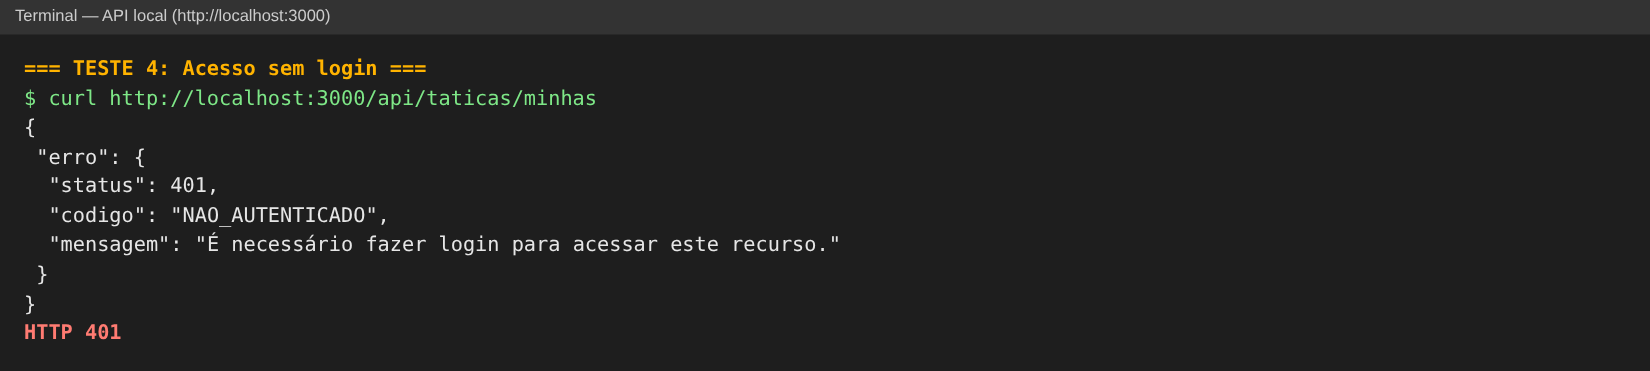
\includegraphics[width=0.9\linewidth]{../evidencias/capturas/seg_05.png}
\caption{Teste 4: acesso a rota protegida sem login}
\end{figure}

\begin{figure}[H]
\centering
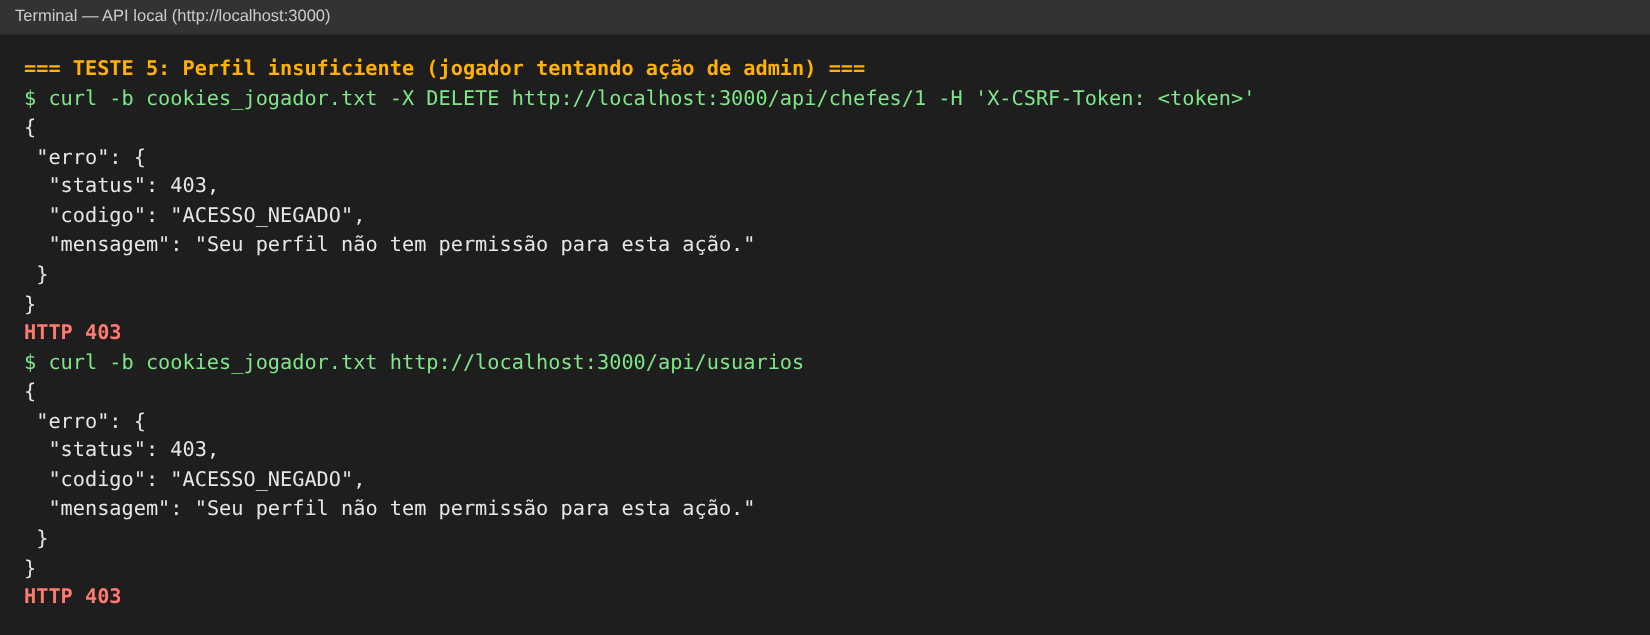
\includegraphics[width=0.9\linewidth]{../evidencias/capturas/seg_06.png}
\caption{Teste 5: jogador tentando excluir chefe e listar usuários}
\end{figure}

\begin{figure}[H]
\centering
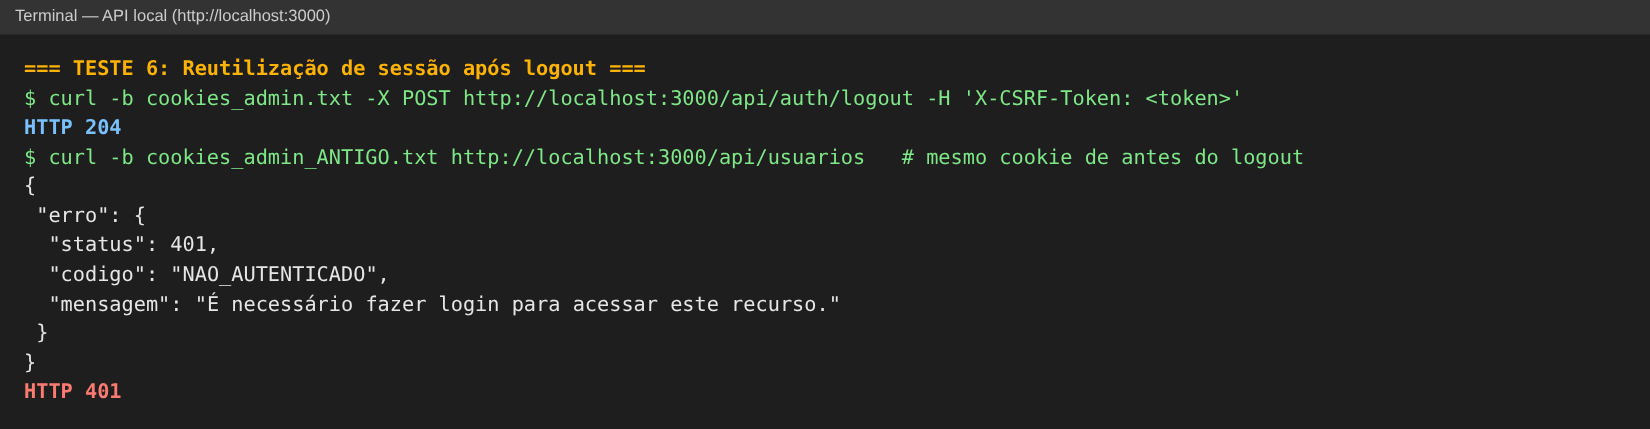
\includegraphics[width=0.9\linewidth]{../evidencias/capturas/seg_07.png}
\caption{Teste 6: o cookie guardado antes do logout não dá mais acesso}
\end{figure}

\begin{figure}[H]
\centering
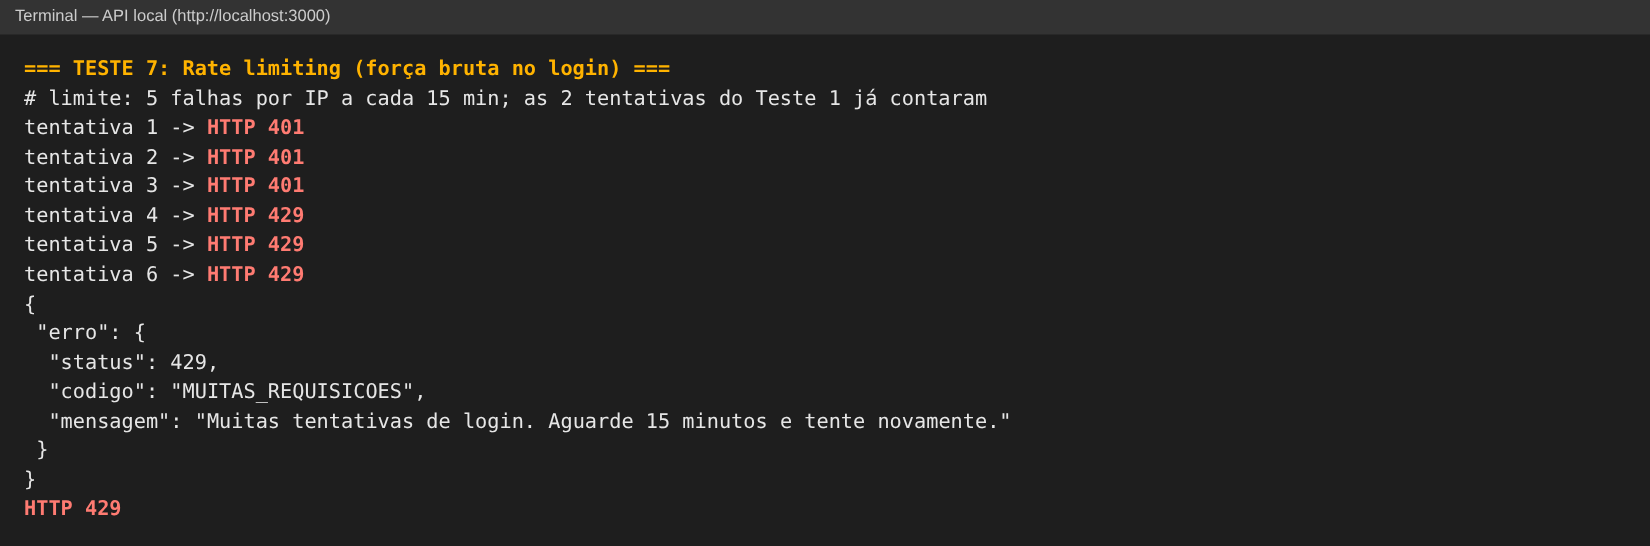
\includegraphics[width=0.9\linewidth]{../evidencias/capturas/seg_08.png}
\caption{Teste 7: rate limiting. O limite é de 5 falhas por IP em 15 minutos; as 2 tentativas do Teste 1 já contaram}
\end{figure}

Além desses, a suíte automatizada verifica que o cadastro ignora
\cod{"perfil": "admin"} (\textit{mass assignment}), que o banco guarda apenas hashes
bcrypt (\cod{\$2b\$...}), que nenhuma resposta contém o campo de senha e que o
stack trace não aparece fora do modo de desenvolvimento.

% =====================================================================
\section{Logs e observabilidade}

O módulo \cod{config/logger.js} grava cada evento como uma linha JSON no arquivo
\cod{backend/logs/app.log} (e no console). Toda linha tem \cod{timestamp} no
formato ISO-8601 (UTC), nível (\cod{debug}, \cod{info}, \cod{aviso}, \cod{erro}),
nome do evento e contexto. Campos como \cod{senha}, \cod{token} e \cod{cookie} são
descartados automaticamente antes da gravação.

\begin{table}[H]
\centering
\caption{Eventos registrados}
\small
\begin{tabularx}{\linewidth}{@{}l l >{\raggedright\arraybackslash}X@{}}
\toprule
Evento & Nível & Quando \\
\midrule
\cod{auth.login\_sucesso} & info & Login aceito (usuário, perfil, IP) \\
\cod{auth.login\_falha} & aviso & Credenciais erradas (e-mail, IP, motivo) \\
\cod{auth.logout} & info & Sessão encerrada \\
\cod{entidade.criada} & info & Usuário, chefe ou tática criados \\
\cod{entidade.atualizada} / \cod{excluida} & info & Alterações e exclusões \\
\cod{erro.interno} & erro & Falha inesperada (mensagem, stack, rota, \cod{requisicaoId}) \\
\cod{acesso.negado} & aviso & Respostas 401/403 por falta de permissão \\
\cod{seguranca.csrf\_invalido} & aviso & Token CSRF ausente ou diferente \\
\cod{seguranca.rate\_limit} & aviso & Limite de requisições atingido \\
\cod{servidor.iniciado} / \cod{encerrando} & info & Ciclo de vida do processo \\
\cod{http.requisicao} & debug & Método, rota, status e duração de cada requisição \\
\bottomrule
\end{tabularx}
\end{table}

Cada requisição recebe um identificador único, devolvido no cabeçalho
\cod{X-Request-Id} e no corpo de qualquer erro. Assim, quando um usuário relata um
erro 500, o \cod{requisicaoId} da resposta leva direto à linha do log com a causa.
Linhas reais do log (trecho do Anexo~\ref{anx:logs}; a terceira é a tentativa de SQL Injection do Teste 1, registrada como e-mail inexistente):

\begin{lstlisting}
{"timestamp":"2026-10-14T17:24:15.001Z","nivel":"info","evento":"auth.login_sucesso","usuarioId":2,"perfil":"jogador","ip":"127.0.0.1"}
{"timestamp":"2026-10-14T17:24:17.781Z","nivel":"aviso","evento":"auth.login_falha","email":"admin@cuphead.local","ip":"127.0.0.1","motivo":"senha_incorreta"}
{"timestamp":"2026-10-14T17:24:32.592Z","nivel":"aviso","evento":"auth.login_falha","email":"admin@cuphead.local'--","ip":"127.0.0.1","motivo":"usuario_inexistente"}
{"timestamp":"2026-10-14T17:24:15.045Z","nivel":"info","evento":"entidade.criada","entidade":"tatica","id":1,"chefeId":1,"por":2}
{"timestamp":"2026-10-14T17:27:56.882Z","nivel":"erro","evento":"erro.interno","requisicaoId":"b9c70b6a-5ccb-4876-bfc8-3ecd5bfe2027","metodo":"GET","rota":"/api/saude","usuarioId":null,"mensagem":"connect ECONNREFUSED 127.0.0.1:5432"}
\end{lstlisting}

% =====================================================================
\section{Desempenho e limitações}

\subsection{Medição de desempenho}

O script \cod{npm run bench} sobe a aplicação com o banco de desenvolvimento e usa
o \textbf{autocannon} para disparar carga contra os endpoints de leitura mais
usados (10 conexões simultâneas, 5 segundos por endpoint). Também mede o tempo do
bcrypt. Ambiente: Node.js 22, PostgreSQL 16, mesma máquina.

\begin{table}[H]
\centering
\caption{Resultados do benchmark}
\small
\begin{tabular}{@{}lrrrrr@{}}
\toprule
Endpoint & Req/s & Média & p50 & p99 & Erros \\
 & & (ms) & (ms) & (ms) & \\
\midrule
\cod{GET /api/chefes} & 537 & 18,1 & 16 & 45 & 0 \\
\cod{GET /api/chefes?ilha=2\&busca=the} & 761 & 12,6 & 11 & 35 & 0 \\
\cod{GET /api/chefes/1} & 996 & 9,5 & 9 & 22 & 0 \\
\cod{GET /api/chefes/1/taticas} & 975 & 9,8 & 9 & 19 & 0 \\
\cod{GET /api/conquistas} & 1219 & 7,7 & 7 & 16 & 0 \\
\bottomrule
\end{tabular}
\end{table}

Todas as leituras ficaram abaixo de 50\,ms no percentil 99, sem erros. A listagem
de chefes é a mais lenta porque executa duas consultas (contagem total para a
paginação e a página em si) e uma subconsulta que conta as táticas aprovadas de
cada chefe.

O login é intencionalmente lento: com custo 12, o bcrypt levou cerca de 460\,ms
para verificar uma senha. Esse custo é o que torna inviável testar milhões de
senhas caso o banco vaze, e foi mantido.

\subsection{Limitações}

\begin{itemize}[leftmargin=1.5em]
  \item O \textit{rate limit} é guardado em memória: reiniciar o servidor zera os
  contadores, e com mais de uma instância cada uma teria o seu. Uma versão em
  produção usaria um armazenamento compartilhado (por exemplo, Redis).
  \item A biblioteca \cod{bcryptjs} é JavaScript puro, escolhida para instalar no
  Windows sem compilador; a versão nativa (\cod{bcrypt}) seria cerca de três vezes
  mais rápida.
  \item Localmente o sistema roda em HTTP. Em produção seria necessário HTTPS
  (e \cod{COOKIE\_SECURE=true}).
  \item Não há confirmação de e-mail nem recuperação de senha.
  \item As imagens da galeria continuam vindo de sites externos, como no
  Trabalho I; se algum deles sair do ar, a imagem some.
  \item A contagem de táticas por chefe é feita em uma subconsulta a cada
  listagem; com muitos dados, valeria guardar esse número em uma coluna.
  \item As métricas do Google Lighthouse medidas no Trabalho I não foram refeitas
  para este relatório.
\end{itemize}

% =====================================================================
\section{Uso de IA generativa}

\textbf{Ferramenta utilizada:} Claude (Anthropic), em uma sessão de agente com
acesso ao repositório, ao PostgreSQL e ao terminal. No Trabalho I havia sido usado
o Google Gemini.

\textbf{Finalidade e partes produzidas:} a ferramenta recebeu o enunciado do
Trabalho II, o relatório e o código do Trabalho I e foi usada para planejar e
gerar a maior parte do Trabalho II:

\begin{itemize}[leftmargin=1.5em]
  \item backend completo (configuração, middlewares, rotas, controllers, services,
  repositories e validação);
  \item modelo de dados, migrações e script SQL;
  \item JavaScript do frontend, páginas \cod{conta.html} e \cod{admin.html} e os
  estilos novos, seguindo a identidade visual do Trabalho I;
  \item testes automatizados, script de benchmark e script de demonstração de
  segurança;
  \item documentação (\cod{README.md}, \cod{docs/API.md}, \cod{docs/ARQUITETURA.md},
  \cod{docs/CHECKLIST.md}), capturas de tela e o texto deste relatório.
\end{itemize}

\textbf{Rastreabilidade:} todos os commits do Trabalho II, a partir de
\cod{chore: reorganiza o projeto do T1 na pasta frontend/} (Anexo~\ref{anx:git}),
foram produzidos com apoio da ferramenta. Os commits do Trabalho I (até a tag
\cod{v1.0}) não foram alterados.

\textbf{Problemas encontrados e corrigidos durante o desenvolvimento:} parte do
que a IA gerou precisou de correção depois de executado e testado:

\begin{itemize}[leftmargin=1.5em]
  \item a senha do administrador no \cod{.env} continha \cod{\#}, que o
  \cod{dotenv} interpreta como início de comentário; a senha era cortada e o
  script \cod{criar-admin} falhava. Foi adicionada uma observação no
  \cod{.env.example};
  \item o \textit{reset} das migrações usava \cod{DROP SCHEMA public}, que falha em
  versões do PostgreSQL anteriores à 15 quando o usuário não é dono do schema. Foi
  trocado pela remoção explícita das tabelas do projeto (commit
  \cod{fix(db)});
  \item a primeira versão da migração de dados inseria os chefes fora da ordem do
  guia original;
  \item mensagens como ``Conquista não encontrado'' tinham erro de concordância;
  \item os logs registravam a rota relativa ao roteador (\cod{/}) em vez da rota
  completa (\cod{/api/usuarios});
  \item no celular, o cabeçalho fixo passou a ocupar quase metade da tela depois da
  inclusão da área de login (commit \cod{fix(frontend)}).
\end{itemize}

\textbf{Avaliação crítica:} a IA acelerou muito a produção de código repetitivo
(camadas, documentação de endpoints, testes) e sugeriu proteções que não estavam
explícitas no enunciado, como comparação de senha em tempo constante e
\textit{Content Security Policy}. Por outro lado, vários dos problemas acima só
apareceram quando o sistema foi executado de verdade, o que mostra que o código
gerado não pode ser aceito sem execução e testes. A responsabilidade pela revisão,
pela execução local e pela apresentação do sistema é do estudante.

% =====================================================================
\section{Conclusões}

O \textit{Cuphead Boss Guide} deixou de ser uma página estática e passou a ser uma
aplicação cliente-servidor com dados persistentes, usuários com perfis distintos e
fluxo de colaboração (envio e moderação de táticas). As duas limitações apontadas
no Trabalho I, o formulário sem efeito e o checklist que não salvava, foram
resolvidas.

Do ponto de vista de engenharia, a separação em camadas com injeção de
dependências foi o que permitiu testar a lógica de negócio isoladamente e,
ao mesmo tempo, testar a aplicação completa contra um banco real. As proteções
exigidas (consultas parametrizadas, escape de saída, CSRF e controle de acesso)
foram implementadas e comprovadas por testes automatizados e manuais, e o
tratamento centralizado de erros com identificador de requisição liga cada
resposta de erro à sua linha no log.

Como próximos passos, ficam: HTTPS e implantação em um servidor, \textit{rate
limit} com armazenamento compartilhado, recuperação de senha por e-mail e uma nova
auditoria Lighthouse da interface com os componentes dinâmicos.

% =====================================================================
\newpage
\appendix
\renewcommand{\thesection}{\Alph{section}}
\section*{Anexos}
\addcontentsline{toc}{section}{Anexos}
\addtocontents{toc}{\protect\setcounter{tocdepth}{1}}

% ---------------------------------------------------------------------
\section{Script de criação do banco}
\label{anx:sql}

Arquivo completo: \cod{backend/database/script\_completo.sql}. Abaixo, a migração
de estrutura (\cod{001\_criar\_tabelas.sql}); a migração 002 contém os
\cod{INSERT} dos 19 chefes e 28 conquistas.

\lstinputlisting[language=SQL, basicstyle=\ttfamily\scriptsize]{../../backend/database/migrations/001_criar_tabelas.sql}

% ---------------------------------------------------------------------
\section{Documentação da API}
\label{anx:api}

{\small
\hypertarget{documentauxe7uxe3o-da-api--cuphead-boss-guide}{%
\subsection{Documentação da API --- Cuphead Boss
Guide}\label{documentauxe7uxe3o-da-api--cuphead-boss-guide}}

API REST em JSON servida em \texttt{http://localhost:3000/api}.

\hypertarget{convenuxe7uxf5es}{%
\subsubsection{Convenções}\label{convenuxe7uxf5es}}

\hypertarget{autenticauxe7uxe3o-e-sessuxe3o}{%
\paragraph{Autenticação e sessão}\label{autenticauxe7uxe3o-e-sessuxe3o}}

\begin{itemize}
\tightlist
\item
  A autenticação é por \textbf{sessão} (cookie \texttt{cuphead.sid},
  \texttt{HttpOnly}, \texttt{SameSite=Strict}).
\item
  O navegador envia o cookie automaticamente; ferramentas como
  \texttt{curl} precisam guardá-lo
  (\texttt{-c\ cookies.txt\ -b\ cookies.txt}).
\end{itemize}

\hypertarget{proteuxe7uxe3o-csrf}{%
\paragraph{Proteção CSRF}\label{proteuxe7uxe3o-csrf}}

Toda requisição \texttt{POST}, \texttt{PUT}, \texttt{PATCH} ou
\texttt{DELETE} precisa do cabeçalho \texttt{X-CSRF-Token} com o token
obtido em \texttt{GET\ /api/auth/sessao}. O login devolve um
\textbf{token novo}, que deve substituir o anterior.

\hypertarget{formato-das-respostas}{%
\paragraph{Formato das respostas}\label{formato-das-respostas}}

Sucesso:

\begin{Verbatim}[breaklines,breakanywhere,fontsize=\scriptsize]
{ "dados": { ... } }
\end{Verbatim}

Listagens paginadas incluem \texttt{paginacao}:

\begin{Verbatim}[breaklines,breakanywhere,fontsize=\scriptsize]
{ "dados": [ ... ], "paginacao": { "pagina": 1, "limite": 6, "total": 19, "totalPaginas": 4 } }
\end{Verbatim}

Erro (todas as rotas):

\begin{Verbatim}[breaklines,breakanywhere,fontsize=\scriptsize]
{
  "erro": {
    "status": 422,
    "codigo": "VALIDACAO",
    "mensagem": "Os dados enviados são inválidos.",
    "requisicaoId": "2df0b9ae-bcc7-4214-8fa4-eb84460f3315",
    "detalhes": [{ "campo": "dificuldade", "mensagem": "deve ser menor ou igual a 5." }]
  }
}
\end{Verbatim}

Com \texttt{NODE\_ENV=development}, erros inesperados (500) também
trazem o bloco \texttt{tecnico} (nome, mensagem original e stack trace).
Em produção esse bloco nunca aparece.

\hypertarget{cuxf3digos-de-status-usados}{%
\paragraph{Códigos de status usados}\label{cuxf3digos-de-status-usados}}

\begin{longtable}[]{@{}llp{0.5\linewidth}@{}}
\toprule\noalign{}
Status & Código (\texttt{erro.codigo}) & Quando \\
\midrule\noalign{}
\endhead
\bottomrule\noalign{}
\endlastfoot
200 & --- & Leitura ou atualização bem-sucedida \\
201 & --- & Recurso criado (cabeçalho \texttt{Location} aponta para
ele) \\
204 & --- & Sucesso sem corpo (logout, exclusão, marcar conquista) \\
400 & \texttt{JSON\_INVALIDO} & Corpo da requisição não é JSON válido \\
401 & \texttt{NAO\_AUTENTICADO} & Rota exige login \\
401 & \texttt{CREDENCIAIS\_INVALIDAS} & E-mail ou senha incorretos \\
403 & \texttt{ACESSO\_NEGADO} & Perfil sem permissão (ver matriz em
\url{ARQUITETURA.md}) \\
403 & \texttt{CSRF\_INVALIDO} & Cabeçalho \texttt{X-CSRF-Token} ausente
ou incorreto \\
404 & \texttt{NAO\_ENCONTRADO} / \texttt{ROTA\_NAO\_ENCONTRADA} &
Registro ou rota inexistente \\
409 & \texttt{CONFLITO} & E-mail/nome duplicado, tática já moderada,
alterar o próprio perfil \\
413 & \texttt{CORPO\_MUITO\_GRANDE} & Corpo maior que 10 KB \\
422 & \texttt{VALIDACAO} & Tipo, tamanho ou formato inválido (lista em
\texttt{detalhes}) \\
429 & \texttt{MUITAS\_REQUISICOES} & Rate limit excedido (login ou
API) \\
500 & \texttt{ERRO\_INTERNO} & Falha inesperada (registrada no log com
\texttt{requisicaoId}) \\
\end{longtable}

\hypertarget{perfis}{%
\paragraph{Perfis}\label{perfis}}

\texttt{visitante} (sem login), \texttt{jogador} (padrão no cadastro) e
\texttt{admin}.

\begin{center}\rule{0.5\linewidth}{0.5pt}\end{center}

\hypertarget{uxedndice}{%
\subsubsection{Índice}\label{uxedndice}}

\begin{longtable}[]{@{}llp{0.5\linewidth}@{}}
\toprule\noalign{}
Método & URL & Acesso \\
\midrule\noalign{}
\endhead
\bottomrule\noalign{}
\endlastfoot
GET & \protect\hyperlink{get-apisaude}{/api/saude} & público \\
GET & \protect\hyperlink{get-apiauthsessao}{/api/auth/sessao} &
público \\
POST & \protect\hyperlink{post-apiauthregistro}{/api/auth/registro} &
público \\
POST & \protect\hyperlink{post-apiauthlogin}{/api/auth/login} & público
(rate limit) \\
POST & \protect\hyperlink{post-apiauthlogout}{/api/auth/logout} &
logado \\
GET & \protect\hyperlink{get-apiauthme}{/api/auth/me} & logado \\
GET & \protect\hyperlink{get-apiilhas}{/api/ilhas} & público \\
GET & \protect\hyperlink{get-apichefes}{/api/chefes} & público \\
GET & \protect\hyperlink{get-apichefesid}{/api/chefes/:id} & público \\
POST & \protect\hyperlink{post-apichefes}{/api/chefes} & admin \\
PUT & \protect\hyperlink{put-apichefesid}{/api/chefes/:id} & admin \\
DELETE & \protect\hyperlink{delete-apichefesid}{/api/chefes/:id} &
admin \\
GET &
\protect\hyperlink{get-apichefesidtaticas}{/api/chefes/:id/taticas} &
público \\
POST & \protect\hyperlink{post-apitaticas}{/api/taticas} & jogador,
admin \\
GET & \protect\hyperlink{get-apitaticasminhas}{/api/taticas/minhas} &
jogador, admin \\
PATCH & \protect\hyperlink{patch-apitaticasid}{/api/taticas/:id} & autor
(tática pendente) \\
DELETE & \protect\hyperlink{delete-apitaticasid}{/api/taticas/:id} &
autor (pendente) ou admin \\
GET & \protect\hyperlink{get-apitaticas}{/api/taticas} & admin \\
PATCH &
\protect\hyperlink{patch-apitaticasidstatus}{/api/taticas/:id/status} &
admin \\
GET & \protect\hyperlink{get-apiconquistas}{/api/conquistas} &
público \\
GET &
\protect\hyperlink{get-apiconquistasprogresso}{/api/conquistas/progresso}
& jogador, admin \\
PUT &
\protect\hyperlink{put-apiconquistasidprogresso}{/api/conquistas/:id/progresso}
& jogador, admin \\
DELETE &
\protect\hyperlink{delete-apiconquistasidprogresso}{/api/conquistas/:id/progresso}
& jogador, admin \\
GET & \protect\hyperlink{get-apiusuarios}{/api/usuarios} & admin \\
PATCH &
\protect\hyperlink{patch-apiusuariosidperfil}{/api/usuarios/:id/perfil}
& admin \\
\end{longtable}

\begin{center}\rule{0.5\linewidth}{0.5pt}\end{center}

\hypertarget{sauxfade}{%
\subsubsection{Saúde}\label{sauxfade}}

\hypertarget{get-apisaude}{%
\paragraph{GET /api/saude}\label{get-apisaude}}

Verifica se a API e o banco estão respondendo.

\textbf{Parâmetros:} nenhum.

\begin{Verbatim}[breaklines,breakanywhere,fontsize=\scriptsize]
curl http://localhost:3000/api/saude
\end{Verbatim}

\begin{Verbatim}[breaklines,breakanywhere,fontsize=\scriptsize]
{ "dados": { "status": "ok", "banco": "ok" } }
\end{Verbatim}

\textbf{Status:} \texttt{200}, \texttt{500} (banco indisponível).

\begin{center}\rule{0.5\linewidth}{0.5pt}\end{center}

\hypertarget{autenticauxe7uxe3o}{%
\subsubsection{Autenticação}\label{autenticauxe7uxe3o}}

\hypertarget{get-apiauthsessao}{%
\paragraph{GET /api/auth/sessao}\label{get-apiauthsessao}}

Retorna o usuário logado (ou \texttt{null}) e o token CSRF da sessão. É
a primeira chamada do frontend.

\textbf{Parâmetros:} nenhum.

\begin{Verbatim}[breaklines,breakanywhere,fontsize=\scriptsize]
curl -c cookies.txt -b cookies.txt http://localhost:3000/api/auth/sessao
\end{Verbatim}

\begin{Verbatim}[breaklines,breakanywhere,fontsize=\scriptsize]
{ "dados": { "usuario": null, "csrfToken": "I8bheqSPZxh4GORdVYSbqZJvIHBMyNJhKqCkg-5M5AM" } }
\end{Verbatim}

\textbf{Status:} \texttt{200}.

\hypertarget{post-apiauthregistro}{%
\paragraph{POST /api/auth/registro}\label{post-apiauthregistro}}

Cria uma conta com perfil \texttt{jogador}. Campos extras (ex.:
\texttt{perfil}) são ignorados.

\textbf{Corpo (JSON):}

\begin{longtable}[]{@{}llp{0.5\linewidth}@{}}
\toprule\noalign{}
Campo & Tipo & Regras \\
\midrule\noalign{}
\endhead
\bottomrule\noalign{}
\endlastfoot
\texttt{nome} & texto & obrigatório, 2--60 caracteres \\
\texttt{email} & texto & obrigatório, e-mail válido, até 254 caracteres
(convertido para minúsculas) \\
\texttt{senha} & texto & obrigatório, 8+ caracteres, letras e números,
até 72 bytes \\
\end{longtable}

\begin{Verbatim}[breaklines,breakanywhere,fontsize=\scriptsize]
curl -b cookies.txt -c cookies.txt -X POST http://localhost:3000/api/auth/registro \
  -H "Content-Type: application/json" -H "X-CSRF-Token: <token>" \
  -d '{"nome":"Cuphead","email":"cup@head.com","senha":"xicara123"}'
\end{Verbatim}

\begin{Verbatim}[breaklines,breakanywhere,fontsize=\scriptsize]
{
  "dados": { "id": 2, "nome": "Cuphead", "email": "cup@head.com", "perfil": "jogador", "criadoEm": "2026-10-14T17:13:40.620Z" }
}
\end{Verbatim}

\textbf{Status:} \texttt{201}, \texttt{403} (CSRF), \texttt{409} (e-mail
já cadastrado), \texttt{422}.

\hypertarget{post-apiauthlogin}{%
\paragraph{POST /api/auth/login}\label{post-apiauthlogin}}

Autentica e cria a sessão. O id de sessão é regenerado (anti-fixação) e
um \textbf{novo token CSRF} é devolvido. Limitado a
\texttt{RATE\_LIMIT\_LOGIN\_MAX} tentativas malsucedidas por IP a cada
\texttt{RATE\_LIMIT\_LOGIN\_JANELA\_MIN} minutos.

\textbf{Corpo (JSON):} \texttt{email} (texto, obrigatório),
\texttt{senha} (texto, obrigatório).

\begin{Verbatim}[breaklines,breakanywhere,fontsize=\scriptsize]
curl -b cookies.txt -c cookies.txt -X POST http://localhost:3000/api/auth/login \
  -H "Content-Type: application/json" -H "X-CSRF-Token: <token>" \
  -d '{"email":"cup@head.com","senha":"xicara123"}'
\end{Verbatim}

\begin{Verbatim}[breaklines,breakanywhere,fontsize=\scriptsize]
{
  "dados": {
    "usuario": { "id": 2, "nome": "Cuphead", "email": "cup@head.com", "perfil": "jogador", "criadoEm": "2026-10-14T17:13:40.620Z" },
    "csrfToken": "RMBNkIqvIVZ8zJvx7kQvLUQUd6Mnrq8bDTWoCPp2sp4"
  }
}
\end{Verbatim}

Credenciais erradas (mesma resposta para e-mail inexistente ou senha
incorreta):

\begin{Verbatim}[breaklines,breakanywhere,fontsize=\scriptsize]
{ "erro": { "status": 401, "codigo": "CREDENCIAIS_INVALIDAS", "mensagem": "E-mail ou senha incorretos.", "requisicaoId": "f387e924-299a-423b-a5b2-50c3b2ecc659" } }
\end{Verbatim}

\textbf{Status:} \texttt{200}, \texttt{401}, \texttt{403} (CSRF),
\texttt{422}, \texttt{429}.

\hypertarget{post-apiauthlogout}{%
\paragraph{POST /api/auth/logout}\label{post-apiauthlogout}}

Destroi a sessão no servidor e apaga o cookie. O cookie antigo deixa de
valer.

\textbf{Parâmetros:} nenhum (exige \texttt{X-CSRF-Token}).

\begin{Verbatim}[breaklines,breakanywhere,fontsize=\scriptsize]
curl -b cookies.txt -c cookies.txt -X POST http://localhost:3000/api/auth/logout -H "X-CSRF-Token: <token>"
\end{Verbatim}

Resposta: corpo vazio.

\textbf{Status:} \texttt{204}, \texttt{401}, \texttt{403} (CSRF).

\hypertarget{get-apiauthme}{%
\paragraph{GET /api/auth/me}\label{get-apiauthme}}

Dados do usuário logado.

\begin{Verbatim}[breaklines,breakanywhere,fontsize=\scriptsize]
curl -b cookies.txt http://localhost:3000/api/auth/me
\end{Verbatim}

\begin{Verbatim}[breaklines,breakanywhere,fontsize=\scriptsize]
{ "dados": { "id": 2, "nome": "Cuphead", "email": "cup@head.com", "perfil": "jogador", "criadoEm": "2026-10-14T17:13:40.620Z" } }
\end{Verbatim}

\textbf{Status:} \texttt{200}, \texttt{401}.

\begin{center}\rule{0.5\linewidth}{0.5pt}\end{center}

\hypertarget{ilhas}{%
\subsubsection{Ilhas}\label{ilhas}}

\hypertarget{get-apiilhas}{%
\paragraph{GET /api/ilhas}\label{get-apiilhas}}

\begin{Verbatim}[breaklines,breakanywhere,fontsize=\scriptsize]
curl http://localhost:3000/api/ilhas
\end{Verbatim}

\begin{Verbatim}[breaklines,breakanywhere,fontsize=\scriptsize]
{
  "dados": [
    { "id": 1, "nome": "Ilha 1", "ordem": 1 },
    { "id": 2, "nome": "Ilha 2", "ordem": 2 },
    { "id": 3, "nome": "Ilha 3", "ordem": 3 },
    { "id": 4, "nome": "Inkwell Hell", "ordem": 4 }
  ]
}
\end{Verbatim}

\textbf{Status:} \texttt{200}.

\begin{center}\rule{0.5\linewidth}{0.5pt}\end{center}

\hypertarget{chefes}{%
\subsubsection{Chefes}\label{chefes}}

Objeto \texttt{Chefe}:

\begin{Verbatim}[breaklines,breakanywhere,fontsize=\scriptsize]
{
  "id": 1,
  "nome": "The Root Pack",
  "fase": "Botanic Panic",
  "estrategia": "O FSM transita de forma linear: Batata (projéteis horizontais), ...",
  "dificuldade": 1,
  "ilhaId": 1,
  "ilhaNome": "Ilha 1",
  "criadoEm": "2026-10-14T17:12:36.512Z",
  "atualizadoEm": "2026-10-14T17:12:36.512Z",
  "totalTaticas": 1
}
\end{Verbatim}

\hypertarget{get-apichefes}{%
\paragraph{GET /api/chefes}\label{get-apichefes}}

Lista paginada, ordenada por ilha.

\textbf{Query string:}

\begin{longtable}[]{@{}lllp{0.42\linewidth}@{}}
\toprule\noalign{}
Parâmetro & Tipo & Padrão & Regras \\
\midrule\noalign{}
\endhead
\bottomrule\noalign{}
\endlastfoot
\texttt{pagina} & inteiro & 1 & ≥ 1 \\
\texttt{limite} & inteiro & 6 & 1--50 \\
\texttt{ilha} & inteiro & --- & id da ilha \\
\texttt{busca} & texto & --- & 1--60 caracteres; procura em nome e fase,
sem diferenciar maiúsculas \\
\end{longtable}

\begin{Verbatim}[breaklines,breakanywhere,fontsize=\scriptsize]
curl "http://localhost:3000/api/chefes?ilha=4&busca=dev"
\end{Verbatim}

\begin{Verbatim}[breaklines,breakanywhere,fontsize=\scriptsize]
{
  "dados": [
    { "id": 19, "nome": "The Devil", "fase": "One Hell of a Time", "estrategia": "Fase 1: Leia os olhos dele ...", "dificuldade": 5,
      "ilhaId": 4, "ilhaNome": "Inkwell Hell", "criadoEm": "...", "atualizadoEm": "...", "totalTaticas": 0 }
  ],
  "paginacao": { "pagina": 1, "limite": 6, "total": 1, "totalPaginas": 1 }
}
\end{Verbatim}

\textbf{Status:} \texttt{200}, \texttt{422} (ex.: \texttt{limite=999}).

\hypertarget{get-apichefesid}{%
\paragraph{GET /api/chefes/:id}\label{get-apichefesid}}

\textbf{Parâmetros de rota:} \texttt{id} (inteiro ≥ 1).

\begin{Verbatim}[breaklines,breakanywhere,fontsize=\scriptsize]
curl http://localhost:3000/api/chefes/1
\end{Verbatim}

Resposta: \texttt{\{\ "dados":\ Chefe\ \}}.

\textbf{Status:} \texttt{200}, \texttt{404}, \texttt{422} (id não
numérico).

\hypertarget{post-apichefes}{%
\paragraph{POST /api/chefes}\label{post-apichefes}}

Somente \textbf{admin}.

\textbf{Corpo (JSON):}

\begin{longtable}[]{@{}llp{0.5\linewidth}@{}}
\toprule\noalign{}
Campo & Tipo & Regras \\
\midrule\noalign{}
\endhead
\bottomrule\noalign{}
\endlastfoot
\texttt{nome} & texto & obrigatório, 2--60, único (sem diferenciar
maiúsculas) \\
\texttt{fase} & texto & obrigatório, 2--80 \\
\texttt{ilhaId} & inteiro & obrigatório, ilha existente \\
\texttt{estrategia} & texto & obrigatório, 20--1000, aceita quebras de
linha \\
\texttt{dificuldade} & inteiro & obrigatório, 1--5 \\
\end{longtable}

\begin{Verbatim}[breaklines,breakanywhere,fontsize=\scriptsize]
curl -b cookies.txt -X POST http://localhost:3000/api/chefes \
  -H "Content-Type: application/json" -H "X-CSRF-Token: <token>" \
  -d '{"nome":"Glumstone the Giant","fase":"Doggone Dogfight","ilhaId":4,"estrategia":"Atire nos olhos e evite as mãos.","dificuldade":4}'
\end{Verbatim}

\begin{Verbatim}[breaklines,breakanywhere,fontsize=\scriptsize]
{
  "dados": { "id": 20, "nome": "Glumstone the Giant", "fase": "Doggone Dogfight", "estrategia": "Atire nos olhos e evite as mãos.",
             "dificuldade": 4, "ilhaId": 4, "ilhaNome": "Inkwell Hell", "criadoEm": "...", "atualizadoEm": "...", "totalTaticas": 0 }
}
\end{Verbatim}

Cabeçalho \texttt{Location:\ /api/chefes/20}.

\textbf{Status:} \texttt{201}, \texttt{401}, \texttt{403}, \texttt{409}
(nome duplicado), \texttt{422}.

\hypertarget{put-apichefesid}{%
\paragraph{PUT /api/chefes/:id}\label{put-apichefesid}}

Somente \textbf{admin}. Substitui todos os campos (mesmo corpo do
\texttt{POST}).

\begin{Verbatim}[breaklines,breakanywhere,fontsize=\scriptsize]
curl -b cookies.txt -X PUT http://localhost:3000/api/chefes/20 \
  -H "Content-Type: application/json" -H "X-CSRF-Token: <token>" \
  -d '{"nome":"Glumstone","fase":"Doggone Dogfight","ilhaId":4,"estrategia":"Estratégia atualizada pelo administrador.","dificuldade":3}'
\end{Verbatim}

Resposta: \texttt{\{\ "dados":\ Chefe\ \}} atualizado.

\textbf{Status:} \texttt{200}, \texttt{401}, \texttt{403}, \texttt{404},
\texttt{409}, \texttt{422}.

\hypertarget{delete-apichefesid}{%
\paragraph{DELETE /api/chefes/:id}\label{delete-apichefesid}}

Somente \textbf{admin}. Remove o chefe e, em cascata, as táticas dele.

\begin{Verbatim}[breaklines,breakanywhere,fontsize=\scriptsize]
curl -b cookies.txt -X DELETE http://localhost:3000/api/chefes/20 -H "X-CSRF-Token: <token>"
\end{Verbatim}

Resposta: corpo vazio.

\textbf{Status:} \texttt{204}, \texttt{401}, \texttt{403}, \texttt{404}.

\hypertarget{get-apichefesidtaticas}{%
\paragraph{GET /api/chefes/:id/taticas}\label{get-apichefesidtaticas}}

Táticas \textbf{aprovadas} do chefe, mais recentes primeiro.

\begin{Verbatim}[breaklines,breakanywhere,fontsize=\scriptsize]
curl http://localhost:3000/api/chefes/1/taticas
\end{Verbatim}

\begin{Verbatim}[breaklines,breakanywhere,fontsize=\scriptsize]
{
  "dados": [
    { "id": 1, "conteudo": "Fique no canto durante a fase da cenoura.", "status": "aprovada", "chefeId": 1, "chefeNome": "The Root Pack",
      "usuarioId": 2, "autorNome": "Cuphead", "criadoEm": "...", "atualizadoEm": "..." }
  ]
}
\end{Verbatim}

\textbf{Status:} \texttt{200}, \texttt{404}, \texttt{422}.

\begin{center}\rule{0.5\linewidth}{0.5pt}\end{center}

\hypertarget{tuxe1ticas-da-comunidade}{%
\subsubsection{Táticas da comunidade}\label{tuxe1ticas-da-comunidade}}

Objeto \texttt{Tatica}: \texttt{id}, \texttt{conteudo}, \texttt{status}
(\texttt{pendente} \textbar{} \texttt{aprovada} \textbar{}
\texttt{rejeitada}), \texttt{chefeId}, \texttt{chefeNome},
\texttt{usuarioId}, \texttt{autorNome}, \texttt{criadoEm},
\texttt{atualizadoEm}.

\hypertarget{post-apitaticas}{%
\paragraph{POST /api/taticas}\label{post-apitaticas}}

Jogador ou admin envia uma tática. Ela nasce \texttt{pendente}.

\textbf{Corpo (JSON):} \texttt{chefeId} (inteiro, chefe existente),
\texttt{conteudo} (texto, 10--1000, aceita quebras de linha).

\begin{Verbatim}[breaklines,breakanywhere,fontsize=\scriptsize]
curl -b cookies.txt -X POST http://localhost:3000/api/taticas \
  -H "Content-Type: application/json" -H "X-CSRF-Token: <token>" \
  -d '{"chefeId":1,"conteudo":"Fique no canto durante a fase da cenoura."}'
\end{Verbatim}

\begin{Verbatim}[breaklines,breakanywhere,fontsize=\scriptsize]
{
  "dados": { "id": 1, "conteudo": "Fique no canto durante a fase da cenoura.", "status": "pendente", "chefeId": 1,
             "chefeNome": "The Root Pack", "usuarioId": 2, "autorNome": "Cuphead", "criadoEm": "...", "atualizadoEm": "..." }
}
\end{Verbatim}

\textbf{Status:} \texttt{201}, \texttt{401}, \texttt{403} (CSRF),
\texttt{422} (inclui chefe inexistente).

\hypertarget{get-apitaticasminhas}{%
\paragraph{GET /api/taticas/minhas}\label{get-apitaticasminhas}}

Todas as táticas do usuário logado (qualquer status).

\begin{Verbatim}[breaklines,breakanywhere,fontsize=\scriptsize]
curl -b cookies.txt http://localhost:3000/api/taticas/minhas
\end{Verbatim}

Resposta: \texttt{\{\ "dados":\ {[}Tatica,\ ...{]}\ \}}.

\textbf{Status:} \texttt{200}, \texttt{401}.

\hypertarget{patch-apitaticasid}{%
\paragraph{PATCH /api/taticas/:id}\label{patch-apitaticasid}}

O \textbf{autor} altera o conteúdo enquanto a tática está
\texttt{pendente}.

\textbf{Corpo (JSON):} \texttt{conteudo} (texto, 10--1000).

\begin{Verbatim}[breaklines,breakanywhere,fontsize=\scriptsize]
curl -b cookies.txt -X PATCH http://localhost:3000/api/taticas/1 \
  -H "Content-Type: application/json" -H "X-CSRF-Token: <token>" \
  -d '{"conteudo":"Conteúdo editado pelo autor enquanto pendente."}'
\end{Verbatim}

Resposta: \texttt{\{\ "dados":\ Tatica\ \}}.

\textbf{Status:} \texttt{200}, \texttt{401}, \texttt{403} (não é o
autor), \texttt{404}, \texttt{409} (já moderada), \texttt{422}.

\hypertarget{delete-apitaticasid}{%
\paragraph{DELETE /api/taticas/:id}\label{delete-apitaticasid}}

O autor exclui a própria tática pendente; o \textbf{admin} exclui
qualquer uma.

\begin{Verbatim}[breaklines,breakanywhere,fontsize=\scriptsize]
curl -b cookies.txt -X DELETE http://localhost:3000/api/taticas/1 -H "X-CSRF-Token: <token>"
\end{Verbatim}

\textbf{Status:} \texttt{204}, \texttt{401}, \texttt{403}, \texttt{404},
\texttt{409}.

\hypertarget{get-apitaticas}{%
\paragraph{GET /api/taticas}\label{get-apitaticas}}

Fila de moderação (somente \textbf{admin}), mais antigas primeiro.

\textbf{Query string:} \texttt{status} (\texttt{pendente} \textbar{}
\texttt{aprovada} \textbar{} \texttt{rejeitada}, opcional),
\texttt{pagina}, \texttt{limite} (padrão 20, máx. 50).

\begin{Verbatim}[breaklines,breakanywhere,fontsize=\scriptsize]
curl -b cookies.txt "http://localhost:3000/api/taticas?status=pendente"
\end{Verbatim}

Resposta:
\texttt{\{\ "dados":\ {[}Tatica,\ ...{]},\ "paginacao":\ \{\ ...\ \}\ \}}.

\textbf{Status:} \texttt{200}, \texttt{401}, \texttt{403}, \texttt{422}.

\hypertarget{patch-apitaticasidstatus}{%
\paragraph{PATCH
/api/taticas/:id/status}\label{patch-apitaticasidstatus}}

Aprova ou rejeita uma tática (somente \textbf{admin}).

\textbf{Corpo (JSON):} \texttt{status} (\texttt{aprovada} \textbar{}
\texttt{rejeitada}).

\begin{Verbatim}[breaklines,breakanywhere,fontsize=\scriptsize]
curl -b cookies.txt -X PATCH http://localhost:3000/api/taticas/1/status \
  -H "Content-Type: application/json" -H "X-CSRF-Token: <token>" -d '{"status":"aprovada"}'
\end{Verbatim}

Resposta: \texttt{\{\ "dados":\ Tatica\ \}} com o novo status.

\textbf{Status:} \texttt{200}, \texttt{401}, \texttt{403}, \texttt{404},
\texttt{422}.

\begin{center}\rule{0.5\linewidth}{0.5pt}\end{center}

\hypertarget{conquistas}{%
\subsubsection{Conquistas}\label{conquistas}}

\hypertarget{get-apiconquistas}{%
\paragraph{GET /api/conquistas}\label{get-apiconquistas}}

Catálogo com as 28 conquistas.

\begin{Verbatim}[breaklines,breakanywhere,fontsize=\scriptsize]
curl http://localhost:3000/api/conquistas
\end{Verbatim}

\begin{Verbatim}[breaklines,breakanywhere,fontsize=\scriptsize]
{ "dados": [ { "id": 1, "nome": "Taking Names", "descricao": "Derrote um chefão." }, "..." ] }
\end{Verbatim}

\textbf{Status:} \texttt{200}.

\hypertarget{get-apiconquistasprogresso}{%
\paragraph{GET
/api/conquistas/progresso}\label{get-apiconquistasprogresso}}

Progresso do usuário logado.

\begin{Verbatim}[breaklines,breakanywhere,fontsize=\scriptsize]
curl -b cookies.txt http://localhost:3000/api/conquistas/progresso
\end{Verbatim}

\begin{Verbatim}[breaklines,breakanywhere,fontsize=\scriptsize]
{ "dados": { "total": 28, "concluidas": 1, "percentual": 4, "itens": [ { "conquistaId": 3, "concluidaEm": "2026-10-14T17:13:41.244Z" } ] } }
\end{Verbatim}

\textbf{Status:} \texttt{200}, \texttt{401}.

\hypertarget{put-apiconquistasidprogresso}{%
\paragraph{PUT
/api/conquistas/:id/progresso}\label{put-apiconquistasidprogresso}}

Marca a conquista como concluída (idempotente: repetir não gera erro).

\begin{Verbatim}[breaklines,breakanywhere,fontsize=\scriptsize]
curl -b cookies.txt -X PUT http://localhost:3000/api/conquistas/3/progresso -H "X-CSRF-Token: <token>"
\end{Verbatim}

\textbf{Status:} \texttt{204}, \texttt{401}, \texttt{403} (CSRF),
\texttt{404}, \texttt{422}.

\hypertarget{delete-apiconquistasidprogresso}{%
\paragraph{DELETE
/api/conquistas/:id/progresso}\label{delete-apiconquistasidprogresso}}

Desmarca a conquista.

\begin{Verbatim}[breaklines,breakanywhere,fontsize=\scriptsize]
curl -b cookies.txt -X DELETE http://localhost:3000/api/conquistas/3/progresso -H "X-CSRF-Token: <token>"
\end{Verbatim}

\textbf{Status:} \texttt{204}, \texttt{401}, \texttt{403} (CSRF),
\texttt{404}, \texttt{422}.

\begin{center}\rule{0.5\linewidth}{0.5pt}\end{center}

\hypertarget{usuuxe1rios-administrauxe7uxe3o}{%
\subsubsection{Usuários
(administração)}\label{usuuxe1rios-administrauxe7uxe3o}}

\hypertarget{get-apiusuarios}{%
\paragraph{GET /api/usuarios}\label{get-apiusuarios}}

Lista paginada de usuários (somente \textbf{admin}). Nunca inclui hash
de senha.

\textbf{Query string:} \texttt{pagina}, \texttt{limite} (padrão 20, máx.
50).

\begin{Verbatim}[breaklines,breakanywhere,fontsize=\scriptsize]
curl -b cookies.txt http://localhost:3000/api/usuarios
\end{Verbatim}

\begin{Verbatim}[breaklines,breakanywhere,fontsize=\scriptsize]
{
  "dados": [ { "id": 1, "nome": "Administrador", "email": "admin@cuphead.local", "perfil": "admin", "criadoEm": "..." } ],
  "paginacao": { "pagina": 1, "limite": 20, "total": 1, "totalPaginas": 1 }
}
\end{Verbatim}

\textbf{Status:} \texttt{200}, \texttt{401}, \texttt{403}, \texttt{422}.

\hypertarget{patch-apiusuariosidperfil}{%
\paragraph{PATCH
/api/usuarios/:id/perfil}\label{patch-apiusuariosidperfil}}

Altera o perfil de outro usuário (somente \textbf{admin}). Vale
imediatamente, inclusive para sessões já abertas.

\textbf{Corpo (JSON):} \texttt{perfil} (\texttt{jogador} \textbar{}
\texttt{admin}).

\begin{Verbatim}[breaklines,breakanywhere,fontsize=\scriptsize]
curl -b cookies.txt -X PATCH http://localhost:3000/api/usuarios/2/perfil \
  -H "Content-Type: application/json" -H "X-CSRF-Token: <token>" -d '{"perfil":"admin"}'
\end{Verbatim}

Resposta: \texttt{\{\ "dados":\ Usuario\ \}} atualizado.

\textbf{Status:} \texttt{200}, \texttt{401}, \texttt{403}, \texttt{404},
\texttt{409} (alterar o próprio perfil), \texttt{422}.

}

% ---------------------------------------------------------------------
\section{Resultado dos testes automatizados}
\label{anx:testes}

\lstinputlisting[basicstyle=\ttfamily\scriptsize, literate={ℹ}{{i}}1]{../evidencias/testes_automatizados.txt}

% ---------------------------------------------------------------------
\section{Capturas da interface}
\label{anx:capturas}

\begin{figure}[H]
\centering
\begin{minipage}[t]{0.48\linewidth}
  \centering
  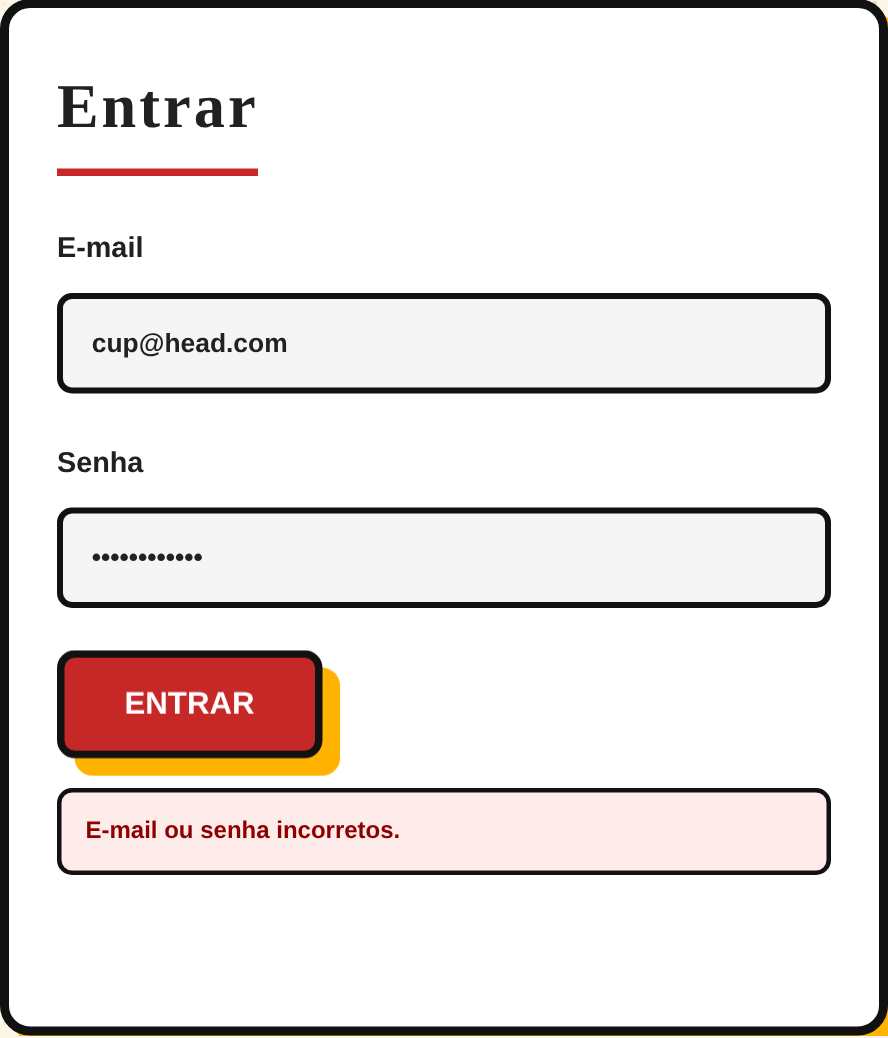
\includegraphics[width=\linewidth]{../evidencias/capturas/02_login_senha_incorreta.png}
  \caption{Login com senha incorreta}
\end{minipage}\hfill
\begin{minipage}[t]{0.48\linewidth}
  \centering
  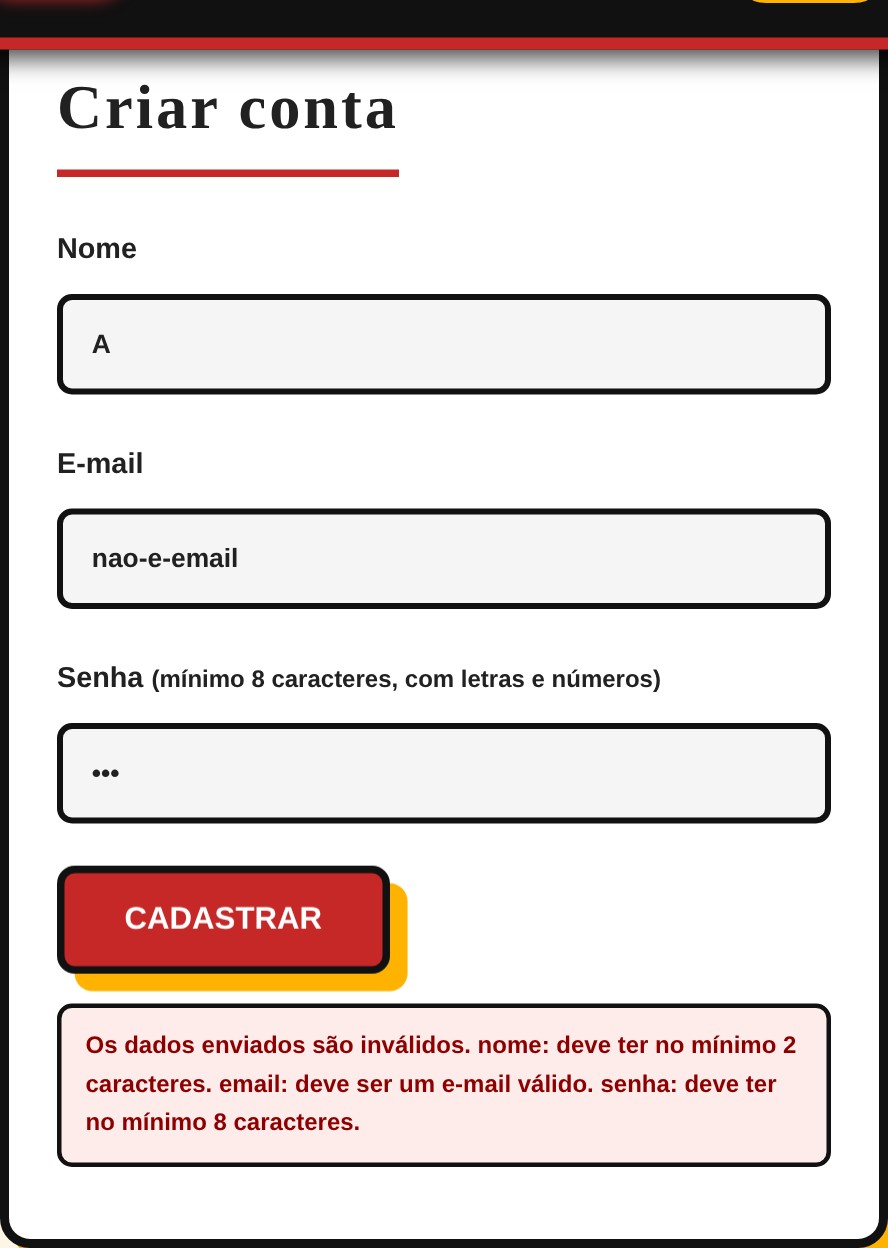
\includegraphics[width=\linewidth]{../evidencias/capturas/03_cadastro_validacao.png}
  \caption{Cadastro com erros de validação devolvidos pela API}
\end{minipage}
\end{figure}

\begin{figure}[H]
\centering
\begin{minipage}[t]{0.48\linewidth}
  \centering
  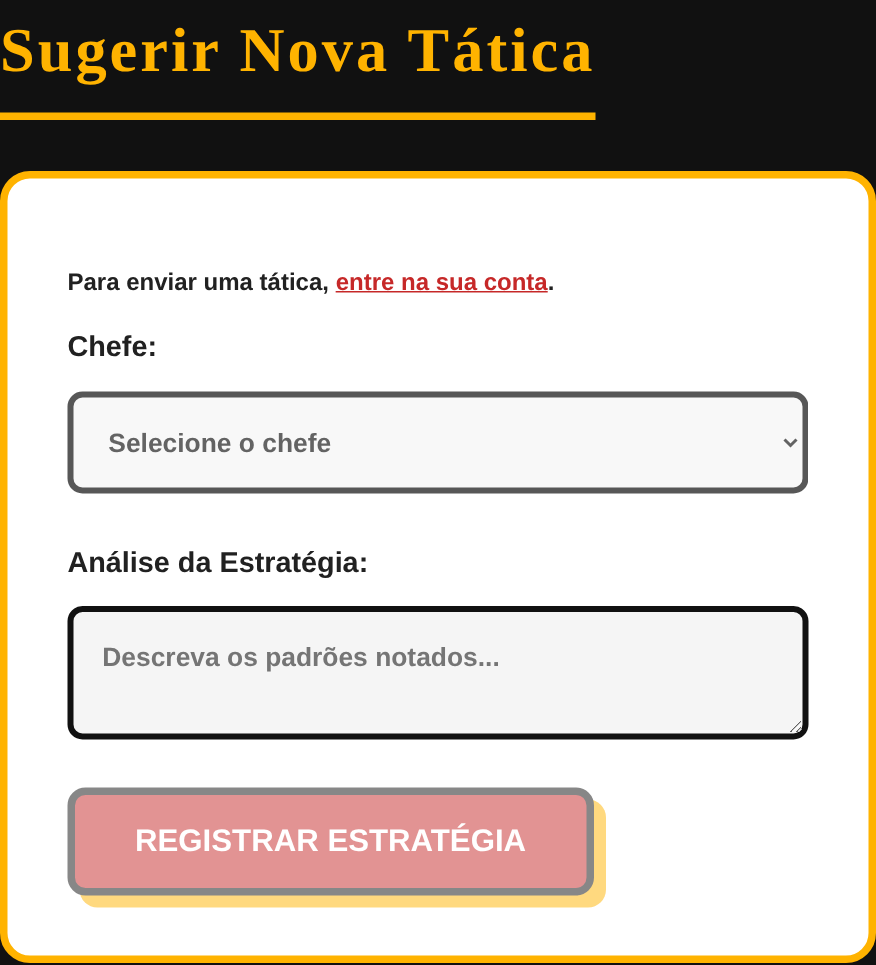
\includegraphics[width=\linewidth]{../evidencias/capturas/01_visitante_formulario_bloqueado.png}
  \caption{Visitante: formulário de tática bloqueado}
\end{minipage}\hfill
\begin{minipage}[t]{0.48\linewidth}
  \centering
  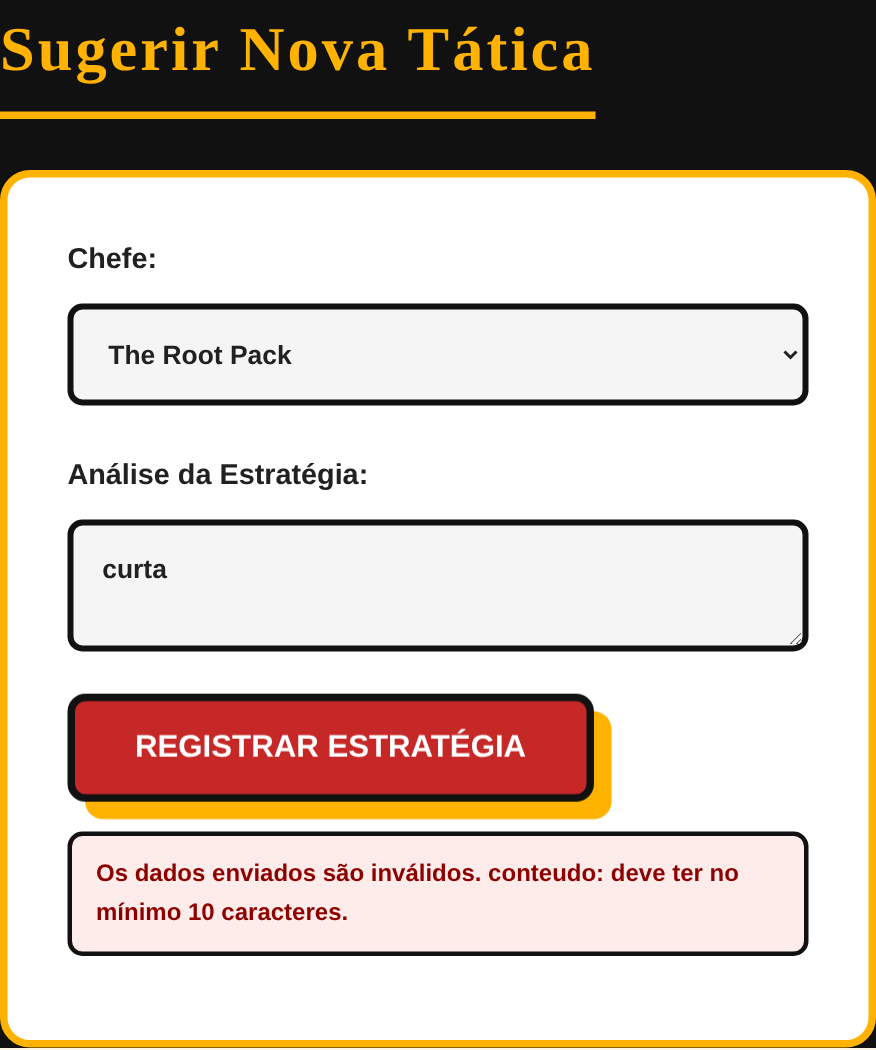
\includegraphics[width=\linewidth]{../evidencias/capturas/06_tatica_validacao.png}
  \caption{Jogador: tática curta demais recusada}
\end{minipage}
\end{figure}

\begin{figure}[H]
\centering
\begin{minipage}[t]{0.36\linewidth}
  \centering
  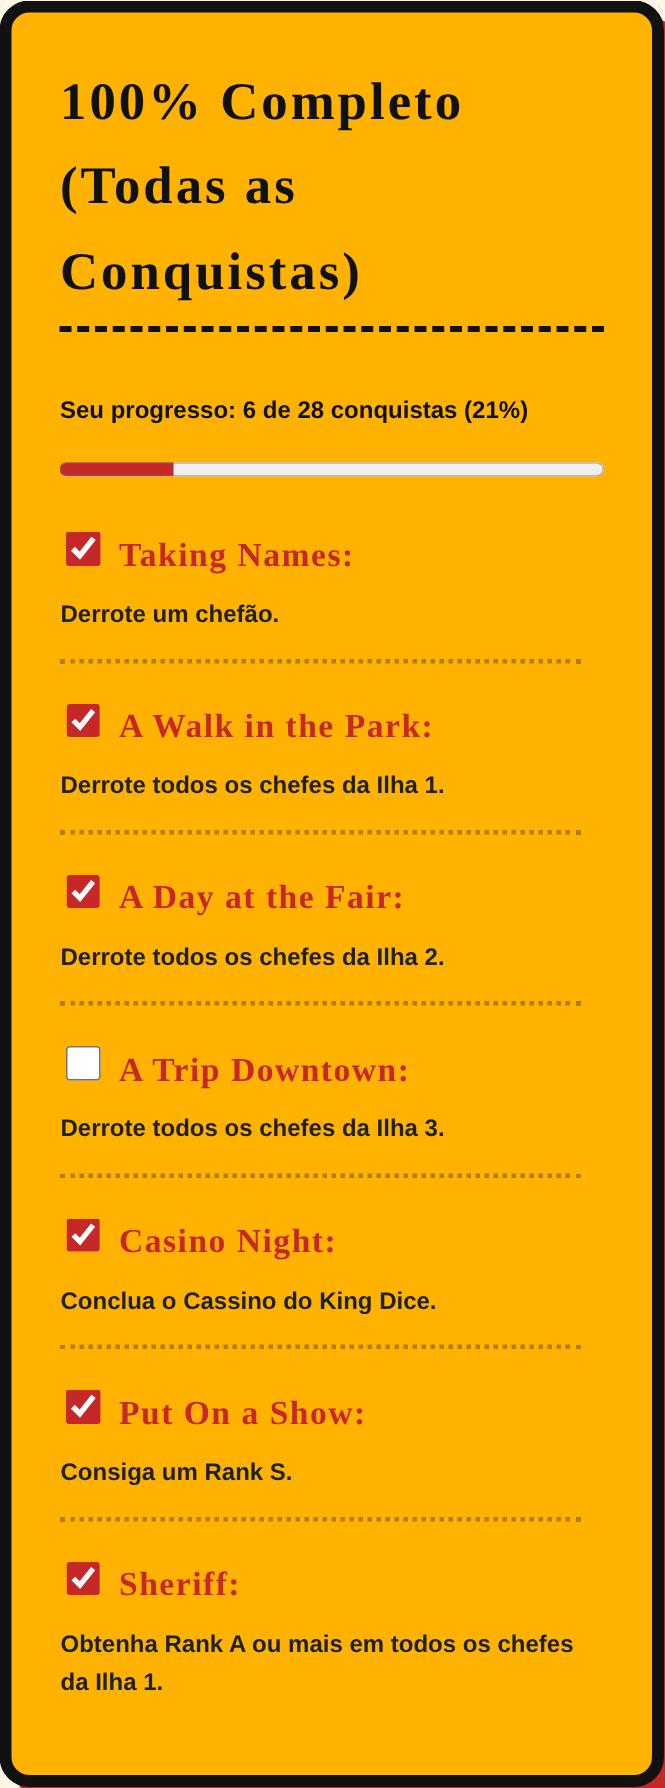
\includegraphics[width=\linewidth]{../evidencias/capturas/05_conquistas_progresso.png}
  \caption{Progresso de conquistas salvo}
\end{minipage}\hfill
\begin{minipage}[t]{0.3\linewidth}
  \centering
  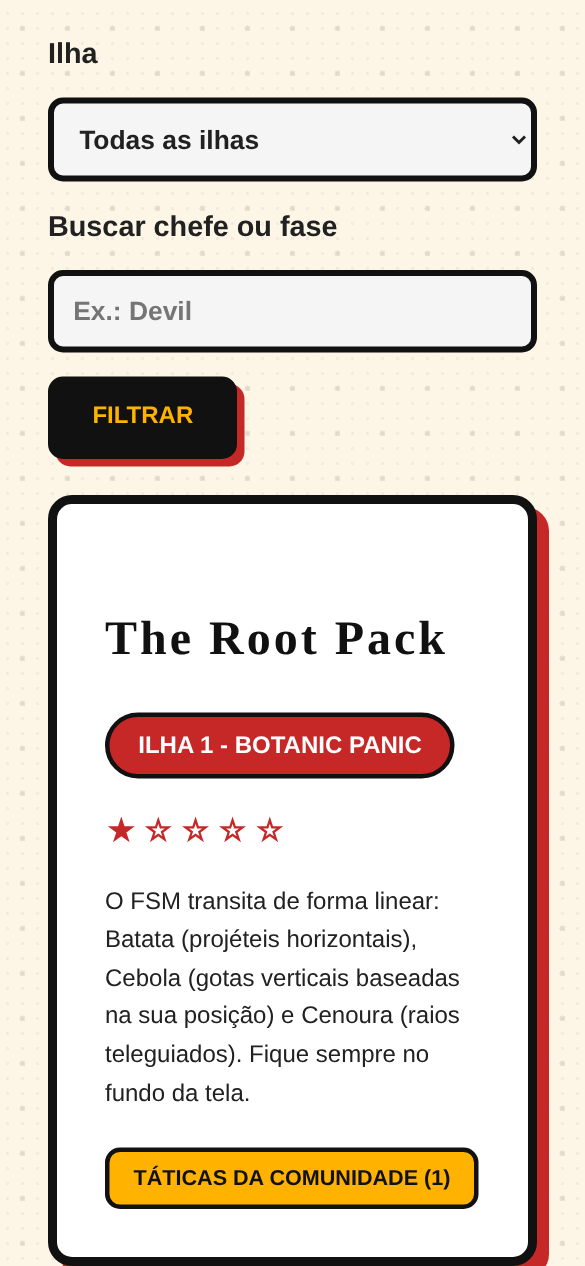
\includegraphics[width=\linewidth]{../evidencias/capturas/12_mobile_chefes.png}
  \caption{Versão mobile (390\,px)}
\end{minipage}
\end{figure}

\begin{figure}[H]
\centering
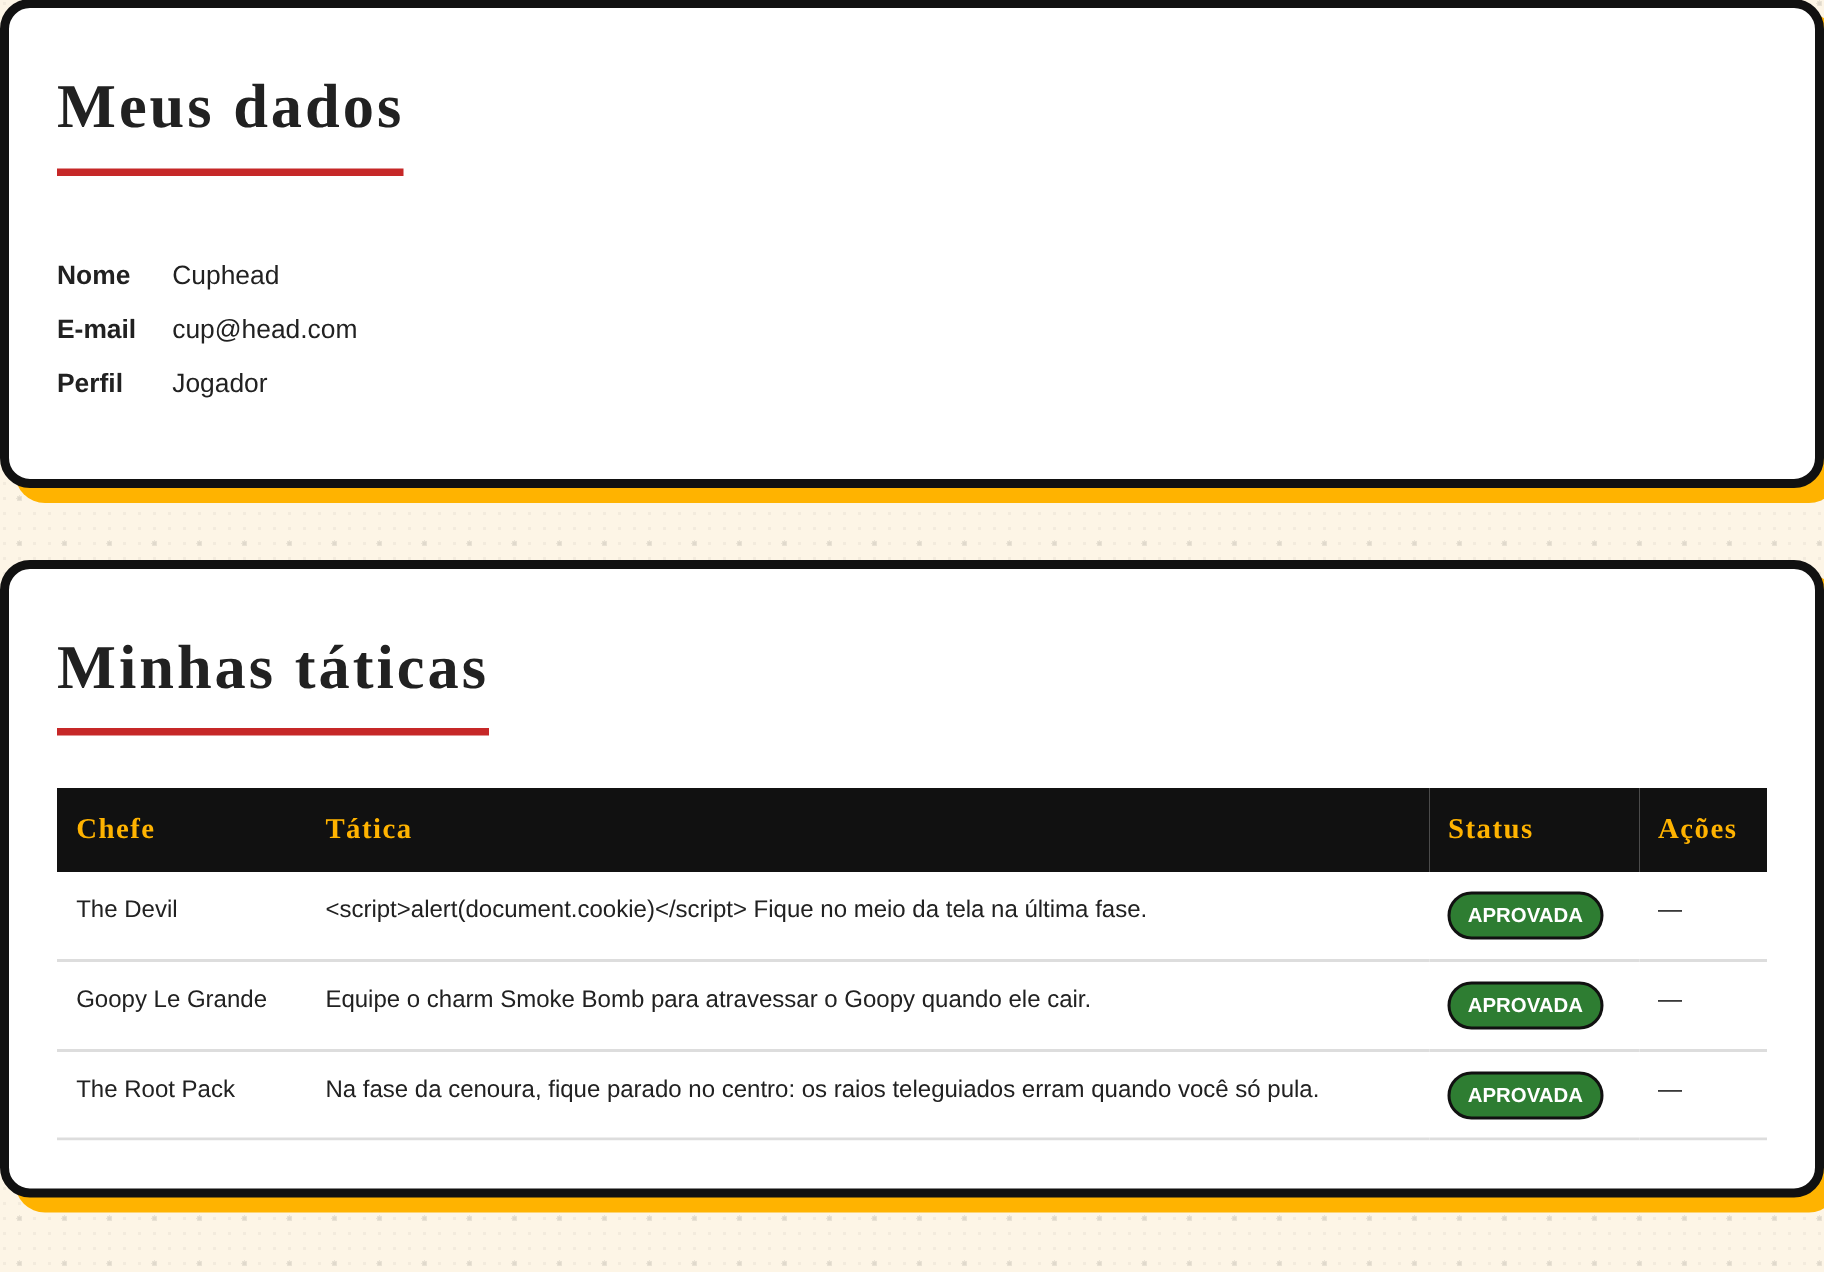
\includegraphics[width=0.85\linewidth]{../evidencias/capturas/08_minha_conta_taticas.png}
\caption{Página ``Minha Conta'' com o status das táticas enviadas}
\end{figure}

\begin{figure}[H]
\centering
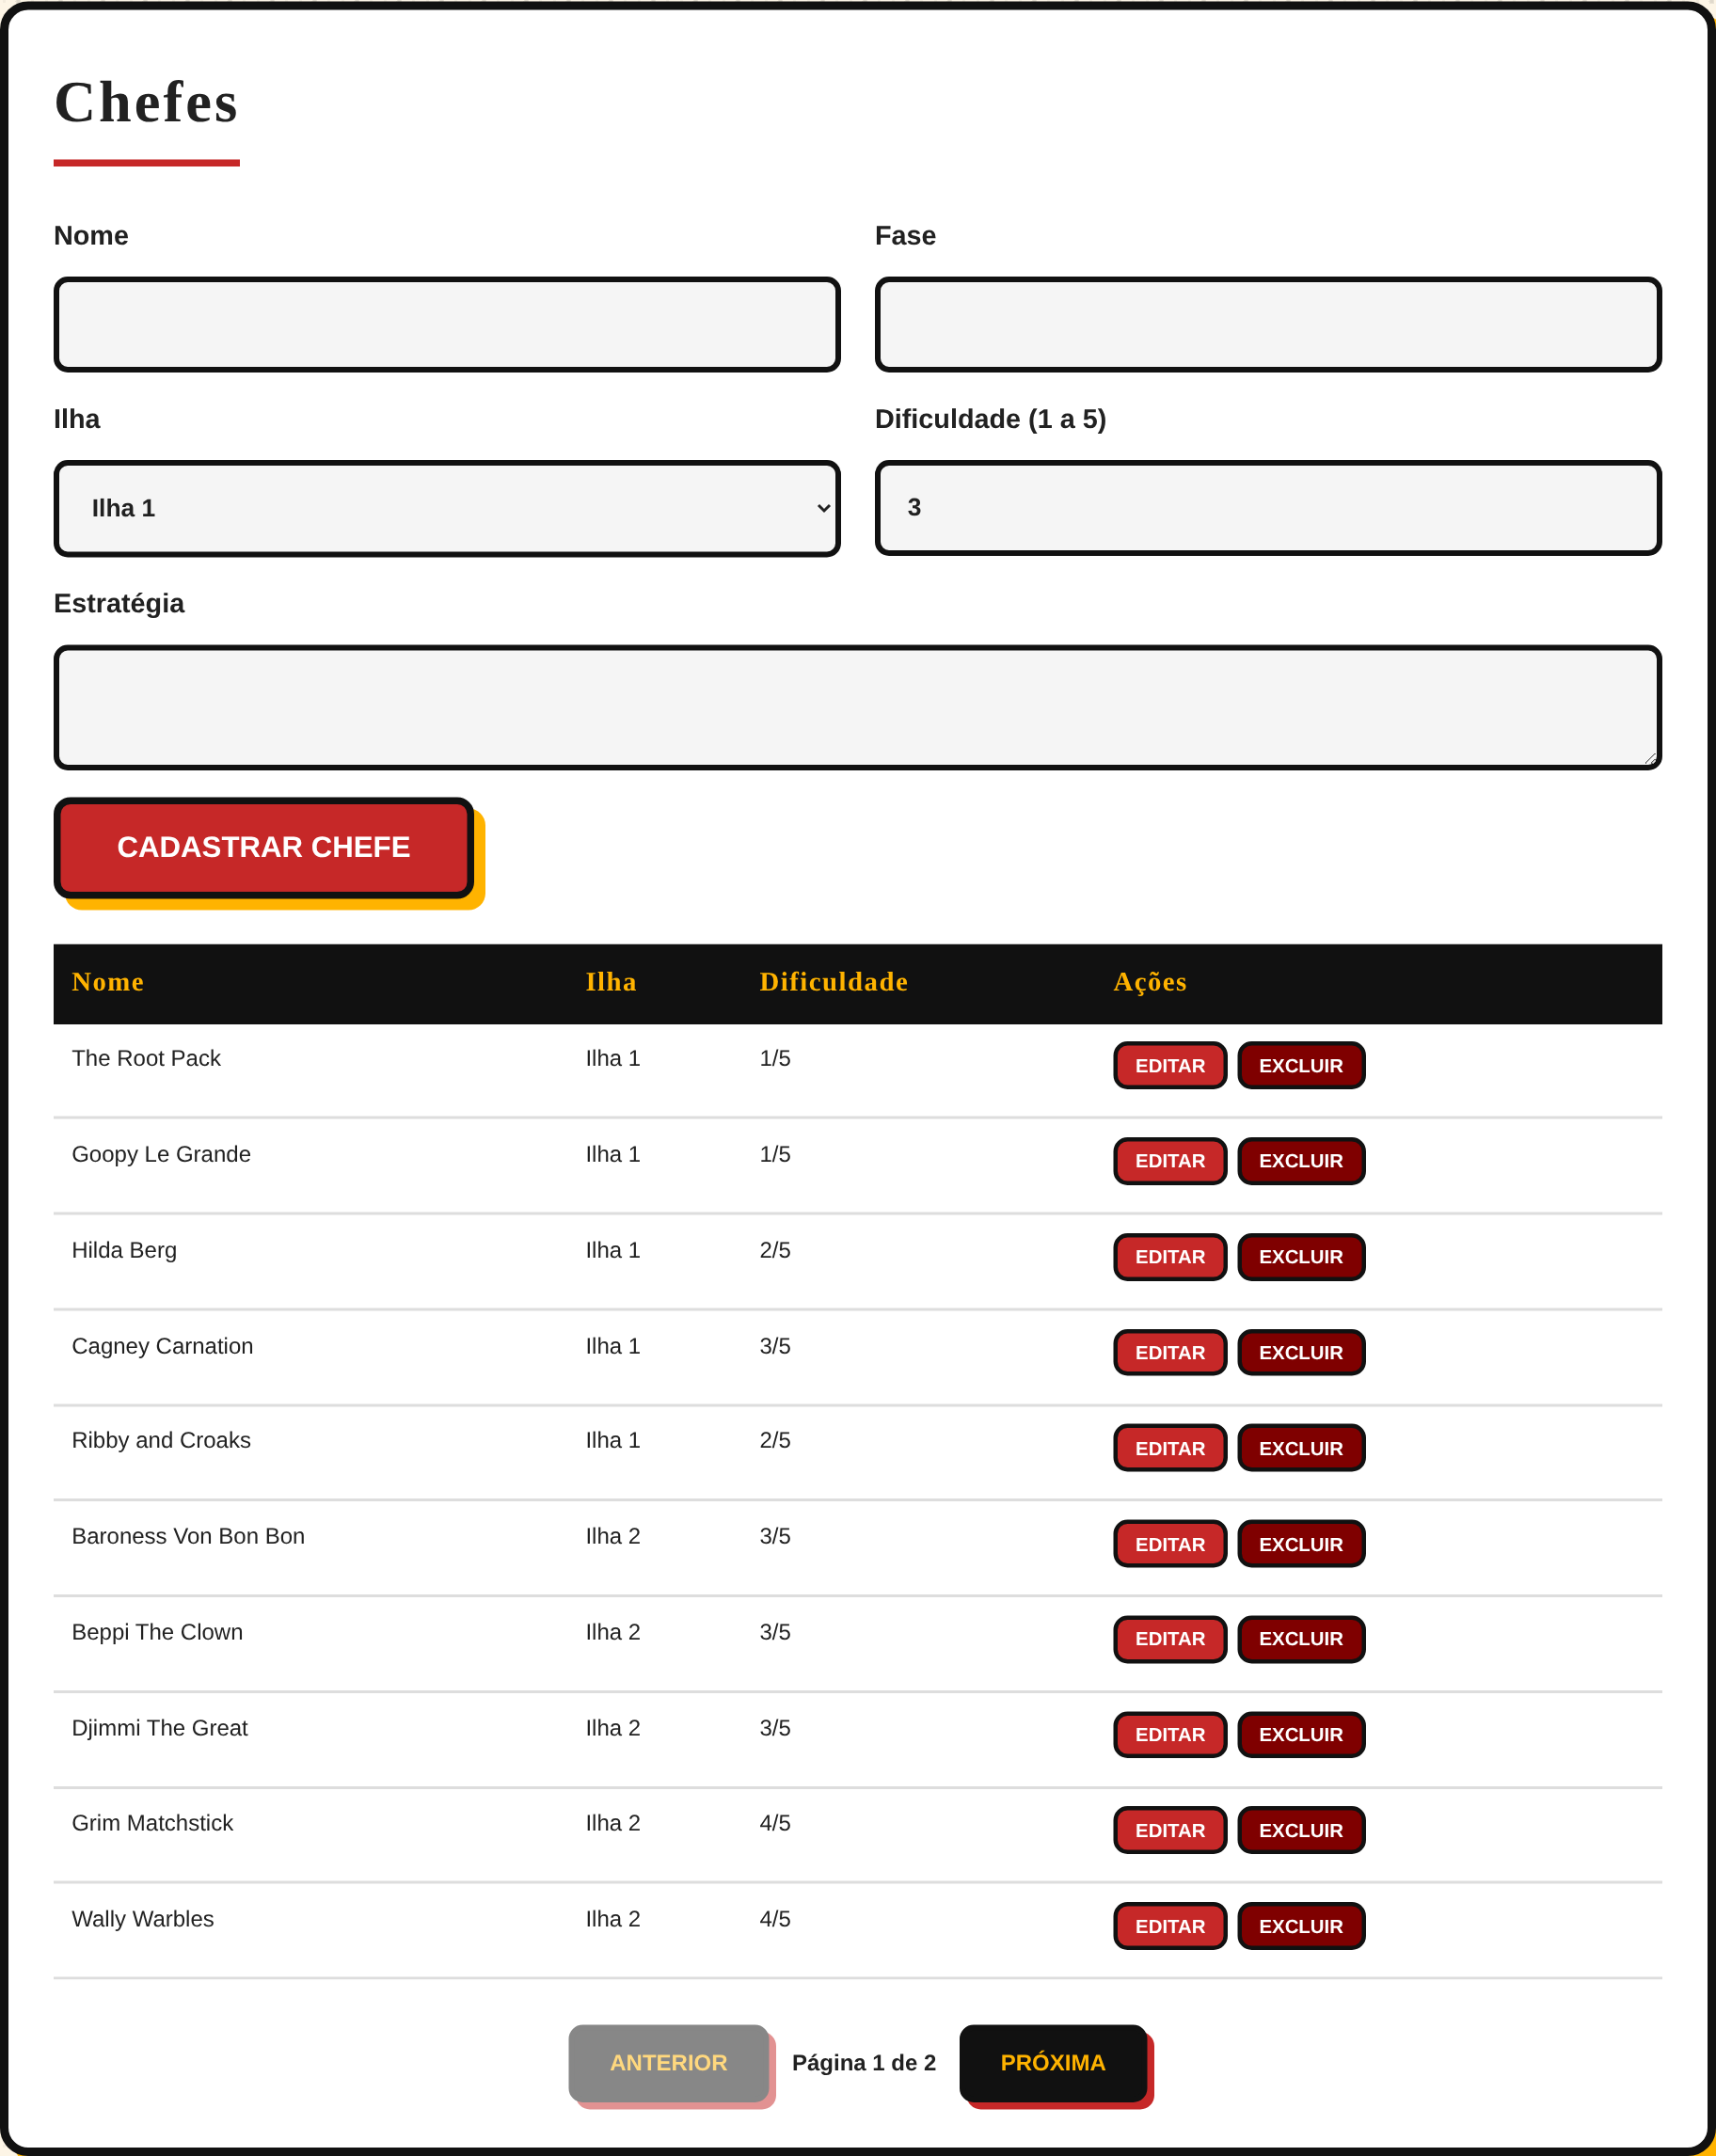
\includegraphics[width=0.75\linewidth]{../evidencias/capturas/09_admin_chefes.png}
\caption{Painel do administrador: CRUD de chefes com paginação}
\end{figure}

\begin{figure}[H]
\centering
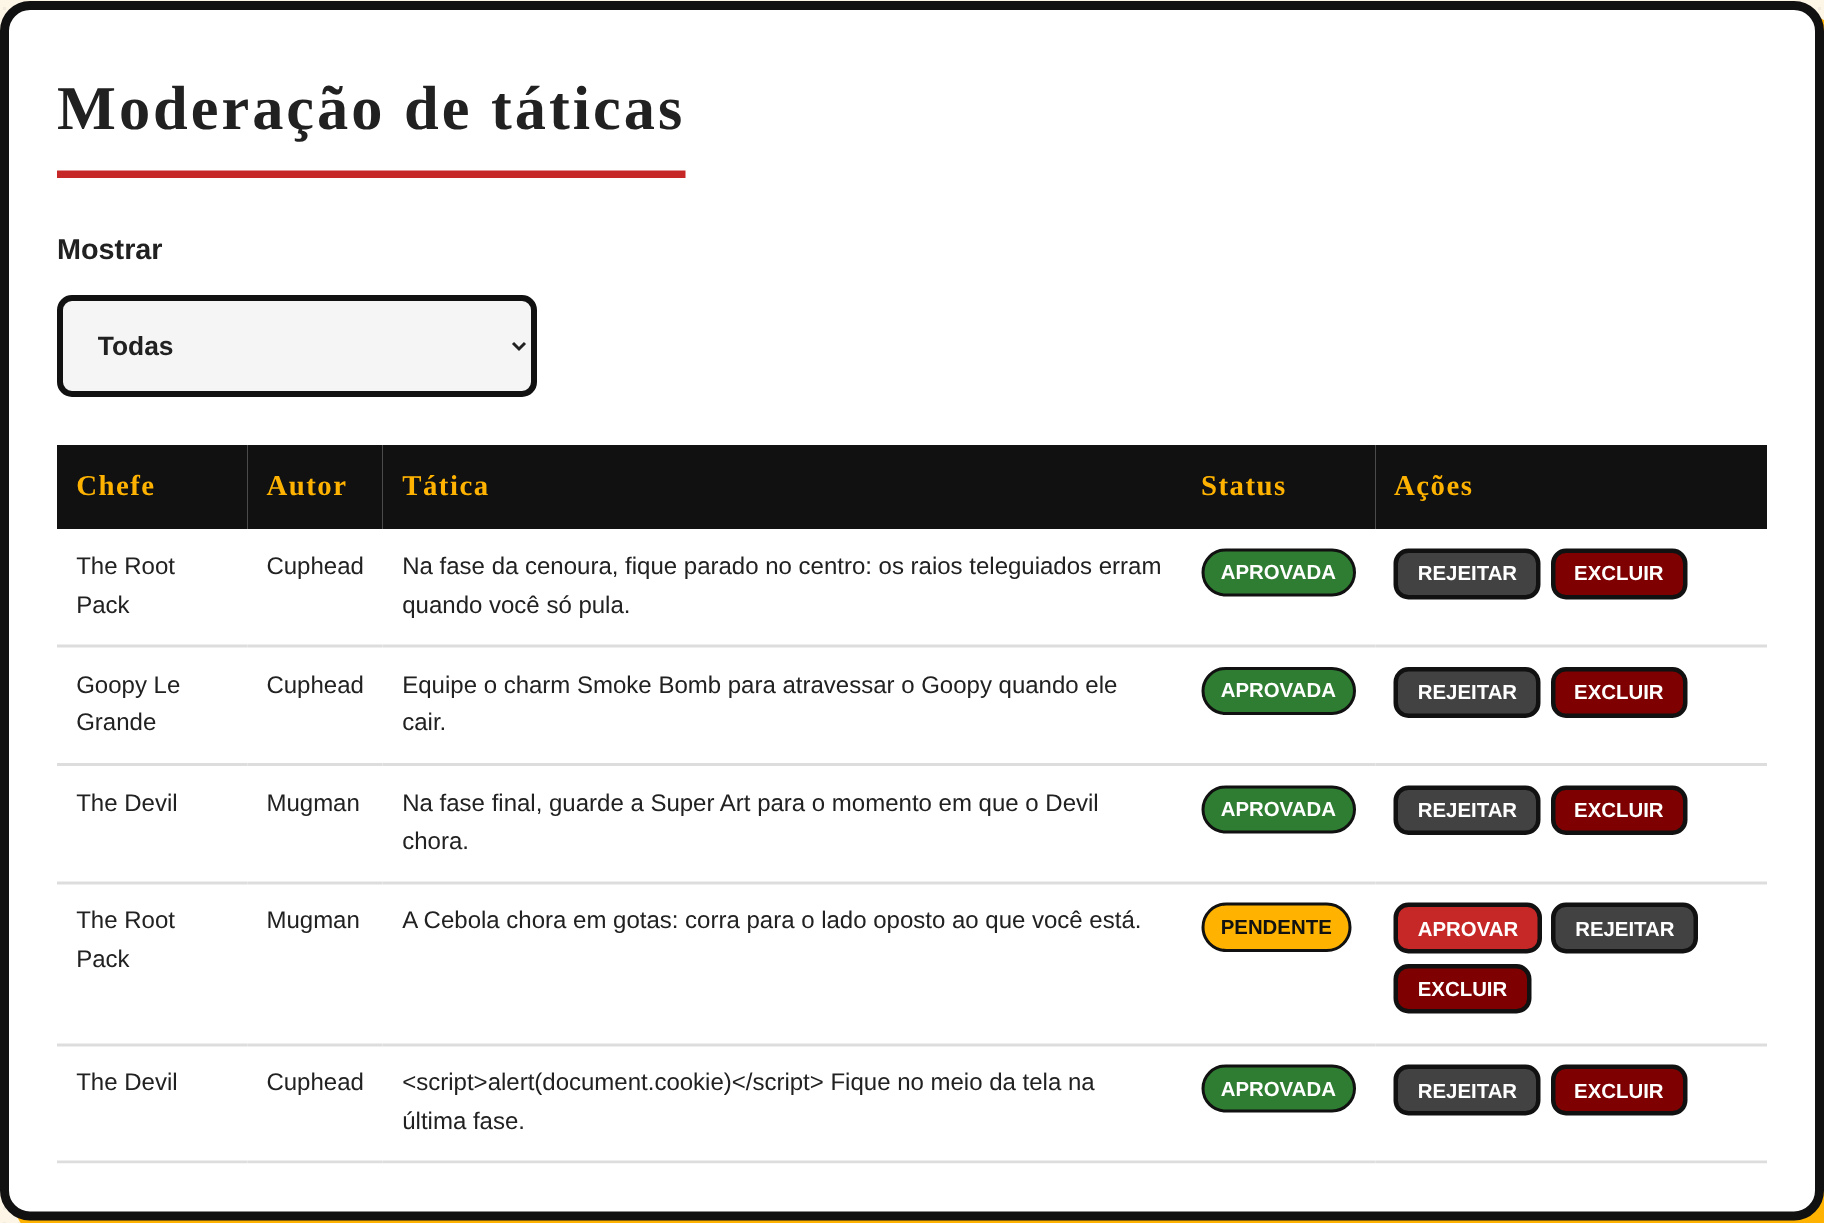
\includegraphics[width=0.85\linewidth]{../evidencias/capturas/10_admin_moderacao.png}
\caption{Painel do administrador: moderação de táticas}
\end{figure}

\begin{figure}[H]
\centering
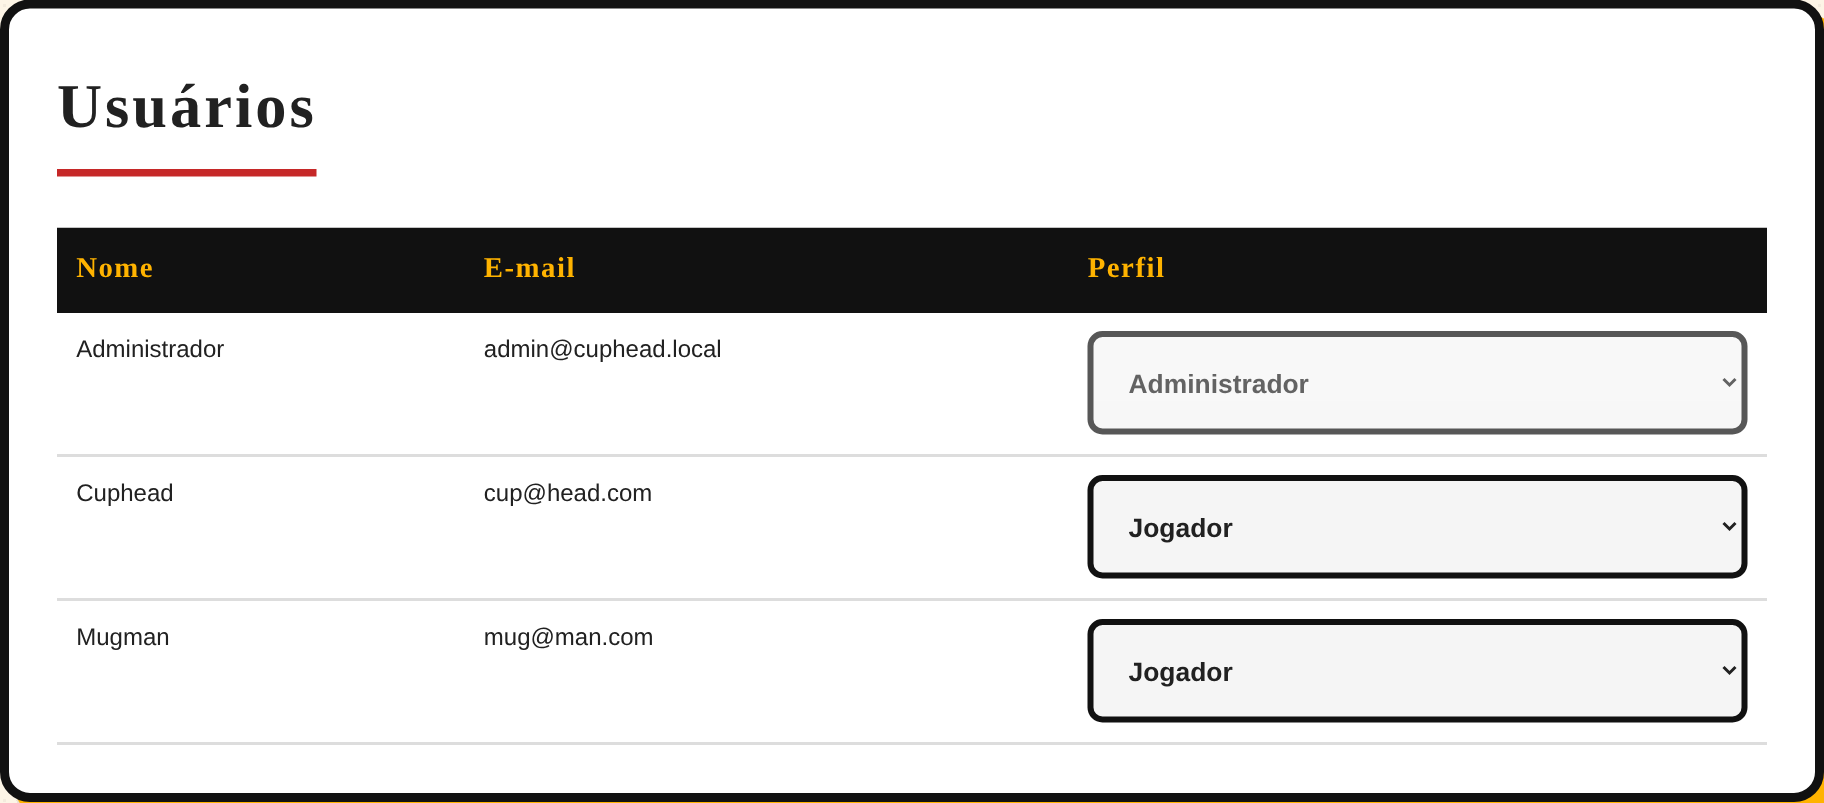
\includegraphics[width=0.85\linewidth]{../evidencias/capturas/11_admin_usuarios.png}
\caption{Painel do administrador: perfis de usuários}
\end{figure}

% ---------------------------------------------------------------------
\section{Amostra dos logs}
\label{anx:logs}

Arquivo \cod{docs/evidencias/logs\_amostra.txt} (até duas linhas de cada tipo de
evento; stack traces encurtados).

\lstinputlisting[basicstyle=\ttfamily\tiny]{../evidencias/logs_amostra.txt}

% ---------------------------------------------------------------------
\section{Histórico Git}
\label{anx:git}

Saída de \cod{git log --oneline --graph --all --decorate}. Fluxo: branches
\cod{feature/*}, \cod{test/*} e \cod{docs/*} integradas em \cod{develop} com
\cod{merge --no-ff}; \cod{develop} integrada em \cod{main}; tags \cod{v1.0}
(Trabalho I) e \cod{v2.0} (Trabalho II). Mensagens no padrão
\textit{Conventional Commits}.

\lstinputlisting[basicstyle=\ttfamily\scriptsize]{../evidencias/git_log.txt}

% ---------------------------------------------------------------------
\section{Checklist de requisitos}
\label{anx:checklist}

\begin{longtable}{@{}>{\raggedright}p{6.2cm}c>{\raggedright\arraybackslash}p{6.4cm}@{}}
\toprule
Requisito & Status & Evidência \\
\midrule
\endhead
1. Separação interface / lógica / dados & \ok & Seção 4 \\
1. Arquitetura documentada & \ok & Seção 4, \cod{docs/ARQUITETURA.md} \\
2. Entidade principal com CRUD & \ok & Chefes; seções 5 e 8 \\
2. Consultas parametrizadas & \ok & \cod{src/repositories/} \\
2. PK, FK, UNIQUE, NOT NULL & \ok & Seção 5, Anexo A \\
2. Script de criação do banco & \ok & \cod{script\_completo.sql} \\
3. Sessão segura & \ok & Seção 6 \\
3. Hash bcrypt & \ok & Seção 6; teste \cod{[Senhas]} \\
3. Logout funcional & \ok & Teste 6 (seção 10) \\
3. Proteção de rotas & \ok & Testes 4 e 5 \\
4. Dois ou mais perfis & \ok & Visitante, jogador, admin \\
4. Matriz de permissões & \ok & Tabela~\ref{tab:matriz} \\
5. Validação de tipo e tamanho & \ok & Seção 7.1 \\
5. Sanitização & \ok & \cod{sanitizarTexto()} \\
5. Erros estruturados & \ok & Seções 7.1 e 7.2 \\
6. SQL Injection & \ok & Testes 1 e 1b \\
6. XSS refletido & \ok & Teste 2, Figura~\ref{fig:xss} \\
6. CSRF & \ok & Teste 3 \\
6. Acesso não autorizado & \ok & Testes 4, 5 e 6 \\
7. Erros padronizados; detalhes só em dev & \ok & Figura~\ref{fig:erro500}; testes automatizados \\
8. Documentação de todos os endpoints & \ok & Anexo B (25 endpoints) \\
9. $\geq$ 5 testes, válidos e inválidos & \ok & 56 testes; Anexo C \\
10. Logs com timestamp (4 eventos) & \ok & Seção 11; Anexo E \\
Opcional: \cod{.env} & \ok & \cod{backend/.env.example} \\
Opcional: migrações & \ok & \cod{database/migrations/} \\
Opcional: paginação & \ok & \cod{?pagina=\&limite=} \\
Opcional: rate limiting & \ok & Teste 7 \\
Opcional: testes de integração & \ok & 22 testes em \cod{tests/integracao/} \\
Git com branches e tags & \ok & Anexo F \\
Sem credenciais no repositório & \ok & Só \cod{.env.example} versionado \\
\bottomrule
\end{longtable}

\end{document}
